\documentclass[parskip=full,11pt]{scrartcl}
\usepackage[utf8]{inputenc}

\title{Simulator für wiederholte Spiele}
\author{Sebastian Feurer, Peter Koepernik, Luc Mercatoris,\\Christian Schorr, Pierre Toussing}

% section numbers in margins:
\renewcommand\sectionlinesformat[4]{\makebox[0pt][r]{#3}#4}

% header & footer
\usepackage{scrlayer-scrpage}
\lofoot{\today}
\refoot{\today}
\pagestyle{scrheadings}

\usepackage[sfdefault,light]{roboto}
\usepackage[T1]{fontenc}
\usepackage[german]{babel}
\usepackage[yyyymmdd]{datetime} % must be after babel
\renewcommand{\dateseparator}{-} % ISO8601 date format
\usepackage{hyperref}
\usepackage{bbm}
\usepackage{amsmath} % for $\text{}$
\usepackage{amssymb}
\usepackage[nameinlink]{cleveref}
\crefname{figure}{Abb}{Abb}
\usepackage[section]{placeins}
\usepackage{xcolor}
\usepackage{graphicx}
\usepackage{subfig}
\usepackage{float} % für Fließumgebungen; Platzierung H verschiebt nicht
\usepackage{multirow}
\restylefloat{figure}
\hypersetup{
	pdftitle={Pflichtenheft},
	bookmarks=true,
}
\usepackage{csquotes}

\newcommand\urlpart[2]{$\underbrace{\text{\texttt{#1}}}_{\text{#2}}$}

\usepackage{pflichtenheft}

\def\adapt{Adaptionsschritt}
\def\adapts{Adaptionsschritte}

\def\segment{Segment}
\def\segments{Segmente}

\usepackage[nonumberlist]{glossaries}

\makenoidxglossaries

\newglossaryentry{Gleichgewicht}
{
	name=Gleichgewicht,
	plural=Gleichgewichte,
	description={Ein Gleichgewicht im Simulationsablauf ist erreicht, wenn keiner der Agenten mehr seine Strategie ändert.}
}

\newglossaryentry{Stufenspiel}
{
	name=Stufenspiel,
	plural=Stufenspiele,
	description={Ein spieltheoretisches Spiel, welches sich als Bimatrix darstellen lässt. (z.B. das Gefangenen-Dilemma)}
}

\newglossaryentry{Bimatrix}
{
	name=Bimatrix,
	plural=Bimatrizen,
	description={Eine Matrix \(A \in (\mathbb{Z} \times \mathbb{Z})^{2 \times 2}\). Ein Stufenspiel wird eindeutig durch die Bimatrix seiner Auszahlungen definiert (siehe Anhang).}
}

\newglossaryentry{Erfolg}
{
	name=Erfolg,
	plural=Erfolge,
	description={Der Erfolg eines Agenten in einer Folge von Runden wird aus dessen Kapitalauszahlungen in diesen Runden berechnet. Er ist Konfigurationsparameter der Simulation. Beispiel ist die Summe aller Auszahlungen.}
}


\newglossaryentry{Kapital}
{
	name=Kapital,
	plural=Kapitale,
	description={Jedem Agenten wird im Laufe einer Wiederholung eine Zahl zugeordnet, die sich aus dem Initialisierungswert zu Beginn der Wiederholung und der Summe der Auszahlungen aus den Stufenspielen der bisherigen Runden zusammensetzt.}
}

\newglossaryentry{Gruppenzugehoerigkeit}
{
	name=Gruppenzugehörigkeit,
	plural=Gruppenzugehörigkeiten,
	description={In einer Simulation sind die Agenten in eine feste, wohldefinierte Anzahl von Gruppen partitioniert. Die Strategien der Agenten können auf Gruppenzugehörigkeiten Bezug nehmen. Dabei haben zwei Agenten genau dann dieselbe Gruppenzugehörigkeit, wenn beide Mitglieder in derselben Gruppe sind. Insbesondere müssen beide Mitglied in einer Gruppe sein.}
}

\newglossaryentry{gruppenloser Agent}
{
	name=gruppenloser Agent,
	plural=gruppenlose Agenten,
	description={Ein Agent, der keiner Gruppe angehört.}
}

\newglossaryentry{Konfiguration}
{
	name=Konfiguration,
	plural=Konfigurationen,
	description={Menge aller variablen Simulationsparameter. Diese sind in den Muss- und Kann-Kriterien aufgelistet.}
}

\newglossaryentry{aktuelle Konfiguration}
{
	name=aktuelle Konfiguration,
	plural=aktuelle Konfigurationen,
	description={Die aktuelle Konfiguration ist die, mit der eine Simulation beim Betätigen des \enquote{Play}-Knopfes gestartet wird.}
}

\newglossaryentry{Nutzer}
{
	name=Nutzer,
	plural=Nutzer,
	description={Eine Person, welche das Programm nutzt.}
}

\newglossaryentry{Multislider}
{
	name=Multislider,
	plural=Multisliders,
	description={Ein Schieberegler mit mehreren möglichen Schiebe-Knöpfen.}
}

\newglossaryentry{Slider-Abschnitt}
{
	name=Slider-Abschnitt,
	plural=Slider-Abschnitte,
	description={Bereich auf dem Slider, der nach rechts und links durch den nächstgelegensten Schiebe-Knopf bzw. den Rand des Sliders begrenzt wird.}
}

\newglossaryentry{Strategie}
{
	name=Strategie,
	plural=Strategien,
	description={Eine Strategie ist ein boole'scher Ausdruck (dessen Variablen von Spieler A und Gegenspieler B abhängen können), der bei Auswertung für zwei Spieler A und B genau dann wahr ist, wenn A unter Verwendung dieser Strategie beim Spiel gegen B kooperiert. Es folgt eine Liste aller Variablen, die in einer Strategie als Literal vorkommen können:
\begin{itemize}
\item A/B hat (bei bisherigen Spielen zwischen A und B im aktuellen \adapt) immer/nie/letztes Mal/wenigstens einmal kooperiert
\item B hat ein höheres/niedrigeres Absolutkapital als A
\item B hat einen höheren/niedrigeren Rang als A (im aktuellen \adapt)
\item A und B haben dieselbe Gruppenzugehörigkeit
\item A und B haben ähnliches Absolutkapital\footnote{Das Absolutkapital zweier Agenten ist ähnlich, genau dann wenn sich der Rang der Agenten, aufgelistet nach Absolutkapital, höchstens um \(20\%\) der Gesamtzahl aller Agenten unterscheidet.}
\item Die Konstanten true und false
\end{itemize}
Insbesondere sind Tit-for-Tat und Grim mögliche Strategien.}
}

\newglossaryentry{gemischte Strategie}
{
	name=gemischte Strategie,
	plural=gemischte Strategien,
	description={Seien \(S_1,...,S_n\) die in einem Simulationsdurchlauf zugelassenen reinen \Glspl{Strategie}. Eine gemischte Strategie ist dann ein Tupel \((\omega_1,...,\omega_n) \in \{0,\frac{1}{10},...,\frac{9}{10},1\}^n\) mit \(\sum_{i=1}^n \omega_i = 1\). \(\omega_i\) entspricht dann der Wahrscheinlichkeit, in einer Runde mit \Gls{Strategie} \(S_i\) zu spielen.}
}

\newglossaryentry{matching}
{
	name=Matching,
	plural=Matchings,
	description={Ein Matching der Menge \(\{1,...,N\}\) aller Agenten ist eine Menge \(M \subset \{\{i,j\} \subset \{1,...,N\} | i \neq j\}\), sodass gilt: \(\forall i \in \{1,...,N\}: \ |\{A \in M | i \in A\}| = 1\).}
}

\newglossaryentry{Effizienz}
{
	name=Effizienz,
	plural=Effizienzen,
	description={Die Effizienz eines Gleichgewichtes ist ein Maß für die Kooperationsbereitschaft der Agenten im Gleichgewichtszustand. Es bezeichne \(p_{ij}\) für \(i,j \in \{1,...,N\}, i \neq j\) die Wahrscheinlichkeit, dass der \(i\)-te Agent nach finaler Strategie mit dem \(j\)-ten Agenten kooperieren würde\footnote{Sind nur reine Strategien zugelassen, ist also \(p_{ij} \in \{0,1\} \forall i,j \in \{1,...,N\}, i \neq j\). \(N\) ist die Anzahl von Agenten.}. Dann ist die Effizienz \(E \in (0,1)\) definiert durch
\[
E = \frac{1}{N(N - 1)} \sum_{i \neq j} p_{ij}.
\]}
}

\newglossaryentry{Einstellungsdauer}
{
	name=Einstellungsdauer,
	plural=Einstellungsdauern,
	description={Anzahl durchgeführter \adapts\ bis zum Erreichen eines Gleichgewichtszustandes in einer Wiederholung.}
}

\begin{document}
\maketitle

\section{Einleitung}

Ziel dieses Projekts ist die Entwicklung einer Simulationsumgebung für wiederholte Spiele. Sie ist aus wissenschaftlichem Interesse motiviert und für den Einsatz in der Forschung ausgelegt. Die Simulationsumgebung wird verwendet, um das Entstehen von \Gls{Gleichgewicht}szuständen bei wiederholten Spielen mehrerer Agenten zu untersuchen.

Es folgt eine Erläuterung des dem Simulator zugrundeliegenden Ablaufs. Dazu sei auch auf \cref{fig:schema} verwiesen.

Eine Simulation besteht aus mehreren Wiederholungen. Eine Wiederholung beginnt mit der Initialisierung der Agenten mit \Glspl{Strategie}, \Gls{Kapital} und \Gls{Gruppenzugehoerigkeit}. Anzahl der Agenten, Zuweisungsverfahren von Anfangsstrategien und Anfangskapital sowie Gruppeneinteilung werden vom \Gls{Nutzer} spezifiziert. Insbesondere legt der \Gls{Nutzer} die Menge aller möglichen \Glspl{Strategie} fest. Danach folgen wiederholt \adapts, bis sich ein Gleichgewicht eingestellt hat oder eine konfigurierbare Höchstzahl an \adapts n erreicht ist. Ein \adapt\ besteht aus einer festen Zahl an Runden. In jeder Runde werden zunächst gemäß eines konfigurierbaren Algorithmus' Paare aus Agenten gebildet. Diese spielen dann unter Betrachtung ihrer aktuellen \Gls{Strategie} das der aktuellen Simulation zugrundeliegende \Gls{Stufenspiel}. Nach Ablauf der Runden wird der \Gls{Erfolg} jedes Agenten in den zurückliegenden Runden quantifiziert und daraus eine Rangliste aller Agenten erstellt. Die Agenten passen nun ihre \Glspl{Strategie} gemäß eines vom \Gls{Nutzer} spezifizierbaren Adaptionsmechanismus an. Ziel dabei ist nicht die Maximierung des Absolutkapitals, sondern eine möglichst hohe Position auf der Rangliste.\newline
Nachdem alle Wiederholungen abgeschlossen sind, erfolgt die Ausgabe der Simulationsergebnisse.

\begin{figure}
	\centering
	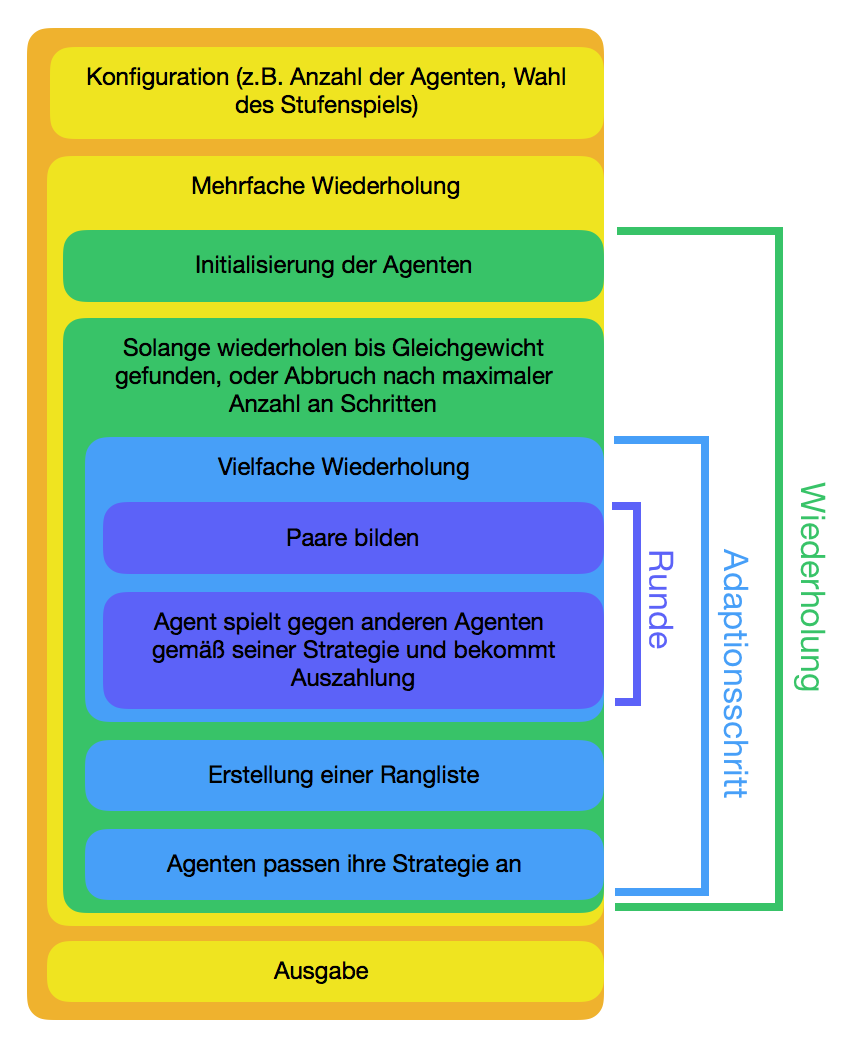
\includegraphics[width=0.9\textwidth]{images/Schema.png}
	\caption{\label{fig:schema}
		Zum Simulationsablauf}
\end{figure}

\pagebreak
\section{Kriterien}
% Diese Section sollte kurz und knapp "für Manager" sein
% und auf eine Seite passen.

\subsection{Muss}

\criterium{Starten einer Simulation}{crt:startsim}

Der \Gls{Nutzer} kann eine Simulation starten, welche dann mit der aktuell gewählten \Gls{Konfiguration} durchgeführt wird.

\criterium{Ausgabe der Simulationsergebnisse}{crt:simresults_std}

Nach Durchführung einer Simulation werden dem \Gls{Nutzer} Informationen über Gleichgewichtshäufigkeit sowie \Gls{Effizienz} und \Gls{Einstellungsdauer} der erreichten Gleichgewichte in den zugehörigen Wiederholungen angezeigt. Weiter können Strategie- und Kapitalverteilungen am Ende der einzelnen Wiederholungen eingesehen werden.

\criterium{Abbrechen einer Simulation}{crt:cancelsim}

Der \Gls{Nutzer} kann eine laufende Simulation abbrechen.

\criterium{Festlegung von Simulationsparametern}{crt:simparam_std}

Der \Gls{Nutzer} hat die Möglichkeit, die folgenden Simulationsparameter festzulegen:
\begin{itemize} \itemsep -10pt
\item Anzahl der Agenten
\item zugrundeliegendes Stufenspiel
\item Anzahl pro \adapt\ durchgeführter Runden
\item Anzahl durchgeführter Wiederholungen
\item Menge aller möglichen \Glspl{Strategie}
\item Anzahl verschiedener Gruppen und jeweils Anzahl zugehöriger Agenten
\item Zuweisungsverfahren für initiale \Glspl{Strategie}
\item Zuweisungsverfahren für initiales Kapital
\item Algorithmus zur Bildung von Paaren beim Beginn einer Runde
\item Erfolgsquantifizierung zur Erstellung der Rangliste am Ende eines \adapt s
\item Adaptionsmechanismus, nach dem Agenten am Ende eines \adapt s ihre \Glspl{Strategie} anpassen
\item Maximale Zahl durchzuführender \adapts.
\end{itemize}

\subsection{Kann}

\criteriumOptional{Starten mehrerer Simulationen}{crt:multisim}
Es können mehrere Simulationen gleichzeitig laufen. Das Programm kann währenddessen unverändert verwendet werden und es wird eine Übersicht über alle gestarteten Simulationen und deren Ausführungsstatus angezeigt.

\criteriumOptional{Anpassen der Gleichgewichtsbedingung}{crt:equicondition}
Es können mehrere Kriterien für das Erreichen eines Gleichgewichts im Simulationsablauf verwendet werden.

\criteriumOptional{Erweiterte Gruppenfunktionalität}{crt:groupfunc}
Gruppen und die Menge \gls{gruppenloser Agent}en können jeweils in \segments\ unterteilt werden. Für jedes \segment\ können Zuweisungsverfahren für initiale \Glspl{Strategie} und initiales Kapital separat festgelegt werden.

\criteriumOptional{Speichern und Laden von Konfigurationen}{crt:saveloadconfig}
Eine Konfiguration kann als Datei abgespeichert werden. Eine solche Konfigurationsdatei kann wiederum geladen werden. Außerdem kann die Konfiguration einer bereits abgeschlossenen Simulation als \gls{aktuelle Konfiguration} übernommen werden.

\criteriumOptional{Speichern und Laden von Simulationsergebnissen}
{crt:saveloadsim}
Eine abgeschlossene Simulation kann als Datei abgespeichert werden. Eine solche Datei kann wiederum geladen werden.

\criteriumOptional{Erstellen eigener \Glspl{Strategie}}{crt:createstrat}
Es können eigene \Glspl{Strategie} erstellt werden.

\criteriumOptional{Erstellen eigener Stufenspiele}{crt:creategame}
Es können eigene Stufenspiele erstellt werden.

\criteriumOptional{Multikonfiguration}{crt:multikonf}
Der \Gls{Nutzer} kann eine Menge von Konfigurationen spezifizieren, in denen die Größe eines bestimmten Parameters eine festgelegte Folge von Werten durchläuft. Die so spezifizierten Simulationen werden gleichzeitig gestartet.

\subsection{Abgrenzung}

\criteriumNot{Kein alternativer Simulationsablauf}{crt:not_altsim}
Der zugrundeliegende Ablauf der Simulation, wie in der Einleitung erklärt, kann nicht verändert werden.

\criteriumNot{Keine komplexen Stufenspiele}{crt:not_complexgames}
Als Stufenspiele sind nur solche zugelassen, die sich als \(2 \times 2\) - \Gls{Bimatrix} mit konstanten Koeffizienten darstellen lassen.

\criteriumNot{Lokalisierung}{crt:local}
Die Anwendung soll nur in deutscher Sprache verfügbar sein.

\pagebreak

%%%%%%%%%%%
\section{Funktionale Anforderungen}

\functionality{Konfiguration bearbeiten}{fnc:editConfig}
\fulfills{crt:simparam_std}
Der \Gls{Nutzer} hat die Möglichkeit, die aktuelle Konfiguration zu bearbeiten.

Dazu kann in der Menüleiste des Startfensters der Eintrag \enquote{Datei} \(\rightarrow\) \enquote{Konfiguration bearbeiten} oder der mit einem Zahnrad-Symbol beschriftete Knopf am oberen rechten Ende des Startfensters betätigt werden (siehe \cref{fig:home}). Daraufhin öffnet sich das Konfigurationsfenster, in dem alle variablen Simulationsparameter festgelegt werden können. Wird der \enquote{Bestätigen}-Knopf in der Toolbar des Konfigurationsfensters betätigt, wird das Konfigurationsfenster geschlossen und die festgelegten Parameter als aktuelle Konfiguration übernommen (siehe \cref{fig:konfig}).

\functionality{Festlegung der Anzahl von Agenten}{fnc:agentcount}
\fulfills{crt:simparam_std}
Der \Gls{Nutzer} hat die Möglichkeit, die Anzahl von Agenten in einer Konfiguration festzulegen.

Die gewünschte Zahl kann im Konfigurationsfenster über einen Slider eingestellt werden. Im Textfeld rechts des Sliders wird der eingestellte Zahlenwert angezeigt. Das Festlegen des Wertes ist auch durch direkte Eingabe in das Textfeld möglich, der Slider wird dann automatisch auf die entsprechende Position gesetzt. Zugelassen sind gerade Zahlen zwischen \(2\) und \(10.000\). Voreingestellt sind \(100\) Agenten (siehe \cref{fig:konfig_main}).

\functionality{Festlegung des Stufenspiels}{fnc:selectgame}
\fulfills{crt:simparam_std}
Der \Gls{Nutzer} kann das zugrundeliegende Stufenspiel einer Konfiguration festlegen.

Dazu befindet sich im Konfigurationsfenster ein Dropdown-Menü. Wird dieses angeklickt, so kann ein Stufenspiel aus einer Liste aller im Programm hinterlegten Stufenspiele ausgewählt werden. Rechts des Dropdown-Menüs wird eine kurze Beschreibung des aktuell eingestellten Stufenspiels angezeigt (siehe \cref{fig:konfig_main}).

Abgesehen von selbst erstellten Stufenspielen sind folgende Stufenspiele im Programm hinterlegt (siehe Anhang):
\begin{itemize} \itemsep -10pt
\item Gefangenendilemma
\item Hirschjagd
\item Feiglingsspiel
\item Kampf der Geschlechter
\item Vertrauensspiel
\item Elfmeterschießen
\end{itemize}
Voreingestellt ist das Gefangenendilemma.

\functionality{Festlegung der Anzahl von Runden pro \adapt}{fnc:rounds}
\fulfills{crt:simparam_std}
Der \Gls{Nutzer} hat die Möglichkeit, die Anzahl pro \adapt\ durchgeführter Runden in einer Konfiguration festzulegen.

Wie die Anzahl von Agenten kann die Anzahl von Runden im Konfigurationsfenster mittels Slider bzw. Textfeld eingestellt werden. Zugelassen sind natürliche Zahlen zwischen \(1\) und \(1000\). Voreingestellt sind \(100\) Runden (siehe \cref{fig:konfig_main}).

\functionality{Festlegung der Anzahl von Wiederholungen}{fnc:repeats}
\fulfills{crt:simparam_std}
Der \Gls{Nutzer} hat die Möglichkeit, die Anzahl durchgeführter Wiederholungen in einer Konfiguration festzulegen.

Wie die Anzahl von Agenten kann die Anzahl von Wiederholungen im Konfigurationsfenster mittels Slider bzw. Textfeld eingegeben werden. Zugelassen sind natürliche Zahlen zwischen \(1\) und \(500\). Voreingestellt sind \(100\) Wiederholungen (siehe \cref{fig:konfig_main}).

\functionality{Festlegung der Menge aller möglichen \Glspl{Strategie}}{fnc:stratset}
\fulfills{crt:simparam_std}
Der \Gls{Nutzer} kann in einer Konfiguration die Menge aller \Glspl{Strategie} festlegen, die von Agenten verwendet werden können.

Dazu befindet sich im Konfigurationsfenster ein mit \enquote{Menge aller möglichen \Glspl{Strategie}} betiteltes Dropdown-Menü. Wird auf das Menü geklickt, klappt nach unten eine Liste aller im Programm hinterlegten \Glspl{Strategie} aus. Neben jeder \Gls{Strategie} befindet sich eine Checkbox. Durch Aktivieren der entsprechenden Checkboxen kann die Menge von \Glspl{Strategie} festgelegt werden (siehe \cref{fig:konfig_strat_detail}).

Unter dem Dropdown-Menü befindet sich eine Checkbox mit der Bezeichnung \enquote{\Glspl{gemischte Strategie} zulassen}. Ist diese aktiviert, so können Agenten im Laufe der so konfigurierten Simulation \glspl{gemischte Strategie} entwickeln. Ist die Checkbox deaktiviert, werden nur reine \Glspl{Strategie} verwendet.

Abgesehen von selbst erstellten \Glspl{Strategie} sind folgende \Glspl{Strategie} im Programm hinterlegt (siehe Anhang):
\begin{itemize} \itemsep -10pt
\item Tit-for-Tat
\item Grim
\item Kooperation mit Agenten mit ähnlichem Absolutkapital, ansonsten keine Kooperation
\item Tit-for-Tat mit Agenten mit ähnlichem Absolutkapital, ansonsten keine Kooperation
\item Keine Kooperation mit Agenten mit höherem Absolutkapital, ansonsten Tit-for-Tat
\item Keine Kooperation mit Agenten mit niedrigerem Absolutkapital, ansonsten Tit-for-Tat
\item Kooperation mit Agenten derselben Gruppenzugehörigkeit, ansonsten keine Kooperation
\item Tit-for-Tat mit Agenten derselben Gruppenzugehörigkeit, ansonsten keine Kooperation
\item Immer Kooperation
\item Nie Kooperation
\end{itemize}
Voreingestellt sind Tit-for-Tat, Grim und \enquote{Immer Kooperation}.

\functionality{Festlegung von Anzahl und Größe der Gruppen}{fnc:groups}
\fulfills{crt:simparam_std}
Der \Gls{Nutzer} hat die Möglichkeit, die Anzahl verschiedener Gruppen in einer Konfiguration festzulegen. Weiterhin kann er angeben, wie viele Agenten den einzelnen Gruppen und wie viele Agenten keiner Gruppe zugehörig sind.

Dazu muss im Konfigurationsfenster zu dem Abschnitt \enquote{Gruppeneinstellungen} navigiert werden (siehe \cref{fig:konfig_group}). Voreingestellt sind null Gruppen. Eine neue Gruppe kann durch Betätigen des \enquote{Gruppe hinzufügen}-Knopfes hinzugefügt werden. Jeder Gruppe wird bei Erstellung eine zufällige, unter allen Gruppen eindeutige Farbe zugeordnet. Ist die maximale Anzahl von fünf Gruppen erreicht, ist der \enquote{Gruppe hinzufügen}-Knopf ausgegraut und kann nicht mehr betätigt werden.

Einer Gruppe werden beim Hinzufügen die Hälfte der bis dahin gruppenlosen Agenten zugewiesen. Die Anzahl der Mitglieder einer Gruppe kann über den \Gls{Multislider} links des \enquote{Gruppe hinzufügen}-Knopfes verändert werden. Für jede Gruppe befindet sich ein entsprechend gefärbter Schiebe-Knopf auf dem \Gls{Multislider}. Der \Gls{Slider-Abschnitt} links des Knopfes wird ebenfalls mit der Gruppenfarbe gefärbt. Die relative Größe jeder Gruppe entspricht genau der relativen Größe des entsprechend gefärbten Abschnitts auf dem Slider. Der rechtsgelegenste Abschnitt ist weiß gefärbt und repräsentiert die gruppenlosen Agenten. Über jedem Abschnitt wird die Zahl von Agenten angezeigt, die diesem Abschnitt angehören. Wird durch Verschieben eines Sliders die Größe einer Gruppe verändert, so ändern sich die Größen anderer Gruppen nicht. Beim Vergrößern einer Gruppe sinkt also die Zahl der gruppenlosen Agenten, beim Verkleinern einer Gruppe vergrößert sie sich. Folglich kann keine Gruppe vergrößert werden, wenn bereits alle Agenten einer Gruppe angehören.

Unter dem Slider befindet sich ein Tab-Control-Element mit einem Tab für jede Gruppe und einem Tab für die gruppenlosen Agenten. Jeder Tab fungiert als Konfigurationsabschnitt der entsprechenden Gruppe bzw. der gruppenlosen Agenten. Am rechten Rand des Tabs jeder Gruppe befindet sich ein mit \enquote{X} beschrifteter Knopf. Wird dieser betätigt, wird die entsprechende Gruppe gelöscht. Der Tab der gruppenlosen Agenten wird angezeigt und die Mitglieder der gelöschten Gruppe werden gruppenlos.

\functionality{Einteilung von Gruppen in \segments}{fnc:segments}
\fulfills{crt:groupfunc}
Der \Gls{Nutzer} kann jede Gruppe und die Menge der gruppenlosen Agenten in ein bis fünf \segments\ unterteilen. Für jedes \segment\ können die Zuweisungsverfahren für initiale \Glspl{Strategie} und initiales Kapital separat konfiguriert werden.

Die Unterteilung erfolgt im Konfigurationsabschnitt einer Gruppe bzw. der gruppenlosen Agenten. Am oberen Ende des Abschnittes befindet sich eine Überschrift \enquote{\segment einstellungen}, darunter ein \Gls{Multislider} und ein \enquote{\segment\ hinzufügen}-Knopf (siehe \cref{fig:konfig_group}). Voreingestellt ist ein Segment. Ein neues Segment kann durch Betätigen des \enquote{\segment\ hinzufügen}-Knopfes hinzugefügt werden. Ist die maximale Anzahl von fünf \segments n erreicht, ist der \enquote{\segment\ hinzufügen}-Knopf ausgegraut und kann nicht mehr betätigt werden. Für jedes hinzugefügte Segment erscheint auf dem \Gls{Multislider} ein Schiebe-Knopf. Wie bei den Gruppeneinstellungen entspricht jeder Abschnitt auf dem Slider einem \segment. Durch Verschieben der Schiebe-Knöpfe kann die Größe der \segments\ verändert werden. Unter dem Slider befindet sich ein Tab-Control-Element mit einem Tab pro \segment. Jeder Tab fungiert als Konfigurationsabschnitt für das entsprechende \segment. Der Konfigurationsabschnitt enthält die Einstellungen für das Zuweisungsverfahren für initiale \Glspl{Strategie} und initiales Kapital.

Am rechten Rand des Tabs jedes \segment s befindet sich ein mit \enquote{X} beschrifteter Knopf. Wird dieser betätigt, so wird das entsprechende \segment\ gelöscht. Gibt es nur noch ein \segment, so ist der \enquote{X}-Knopf ausgegraut und kann nicht betätigt werden.

\functionality{Festlegung des Zuweisungsverfahrens für initiale \Glspl{Strategie}}{fnc:initialstrat}
\fulfills{crt:simparam_std}
\fulfills{crt:groupfunc}
Der \Gls{Nutzer} kann das Zuweisungsverfahren für die initialen \Glspl{Strategie} der Agenten beim Beginn einer Wiederholung festlegen. Diese Einstellung findet für jedes \segment\ einer Gruppe und für jedes \segment\ der gruppenlosen Agenten separat statt.

Die Einstellung erfolgt in dem Konfigurationsabschnitt eines \segment s. Dort befindet sich ein mit \enquote{Initiale \Glspl{Strategie}} beschrifteter Unterabschnitt. In diesem befinden sich zwei nebeneinander angeordnete List-Boxen (siehe \cref{fig:konfig_segment})). Die Linke ist beschriftet mit \enquote{Verfügbare \Glspl{Strategie}}, die Rechte mit \enquote{Gewählte \Glspl{Strategie}}. In der linken Box sind zunächst alle \Glspl{Strategie} aufgelistet, die für diese Konfiguration zugelassen sind. Die rechte Box ist zunächst leer. Per üblicher \textsf{CTRL}- und \textsf{SHIFT}-Klick-Funktionalität können eine oder mehrere \Glspl{Strategie} in der linken Box ausgewählt werden. Betätigen des mit \enquote{\(>\)} beschrifteten Knopfes zwischen den beiden Boxen entfernt alle ausgewählten \Glspl{Strategie} aus der linken Box und fügt sie in die rechte Box ein. Analog können \Glspl{Strategie} in der rechten Box ausgewählt und mittels Betätigen des \enquote{\(<\)}-Knopfes aus der rechten Box entfernt und in die Linke eingefügt werden. Betätigen des \enquote{\(\gg\)}-Knopfes entfernt alle \Glspl{Strategie} aus der linken Box und fügt sie in die rechte Box ein. Betätigen des \enquote{\(\ll\)}-Knopfes entfernt alle \Glspl{Strategie} aus der rechten Box und fügt sie in die linke Box ein.

Zu Beginn jeder Wiederholung in einer so konfigurierten Simulation wird jedem Agent aus dem aktuell konfigurierten \segment\ zufällig eine \Gls{Strategie} aus der Liste der gewählten \Glspl{Strategie} zugeordnet. Ist diese Liste leer, werden den Agenten zufällige \Glspl{Strategie} aus der Menge aller möglichen \Glspl{Strategie} zugeordnet. Insbesondere werden Agenten immer mit reinen \Glspl{Strategie} initialisiert.

Eine \Gls{Strategie}, die sich in einem Segment in den \enquote{ausgewählten \Glspl{Strategie}} befindet, kann in den Grundeinstellungen nicht aus der Menge aller möglichen \Glspl{Strategie} entfernt werden. Die entsprechende Checkbox im Dropdown-Menü ist ausgegraut.

\functionality{Festlegung des Zuweisungsverfahrens für initiales Kapital}{fnc:initialcap}
\fulfills{crt:simparam_std}
\fulfills{crt:groupfunc}
Der \Gls{Nutzer} kann das Zuweisungsverfahren für das initiale Kapital der Agenten beim Beginn einer Wiederholung festlegen. Diese Einstellung findet für jedes \segment\ einer Gruppe und für jedes \segment\ der gruppenlosen Agenten separat statt.

Die Einstellung erfolgt in dem Konfigurationsabschnitt eines \segment s. Dort befindet sich ein mit \enquote{Kapitalverteilung} beschrifteter Unterabschnitt (siehe \cref{fig:konfig_cap})). Mittels Radiobuttons kann eine der folgenden Wahrscheinlichkeitsverteilungen gewählt werden:
\begin{itemize}\itemsep -10pt
\item Gleichverteilung
\item Binomialverteilung
\item Poissonverteilung
\end{itemize}
Unter den Radiobuttons befinden sich Eingabemöglichkeiten zur Parametrisierung der aktuell gewählten Verteilung, eine kurze Beschreibung und ein Graph der Verteilung. Voreingestellt ist die Gleichverteilung.

Für die Gleichverteilung müssen die beiden Intervallgrenzen \(a,b \in \mathbb{N}_0, \ a < b\) in Textfeldern angegeben werden. Voreingestellt ist \(a = 0, b = 100\).

Bei der Binomialverteilung müssen die Intervallgrenzen \(a,b \in \mathbb{N}_0, \ a < b\) in Textfeldern und der Parameter \(p \in (0,1)\) mittels Slider angegeben werden. Voreingestellt ist \(a = 0, b = 100, p = 0.5\).

Bei der Poisson-Verteilung muss der Parameter \(\lambda \in \mathbb{N}_0\) in einem Textfeld angegeben werden. Voreingestellt ist \(\lambda = 50\).

Bei fehlerhafter Eingabe eines Parameters wird die Eingabe auf den nächsten zugelassenen Wert abgeändert.

Zu Beginn jeder Wiederholung in einer so konfigurierten Simulation wird jedem Agent aus dem aktuell konfigurierten \segment\ ein zufälliger Betrag aus der festgelegten Wahrscheinlichkeitsverteilung als initiales Kapital zugewiesen.

\functionality{Festlegung des Algorithmus zur Paarbildung}{fnc:algopaar}
\fulfills{crt:simparam_std}

Der \Gls{Nutzer} hat die Möglichkeit, den Algorithmus festzulegen, der die Agenten zu Beginn jeder Runde in Paare einteilt.

Dazu befindet sich im Konfigurationsfenster im Abschnitt \enquote{Erweiterte Einstellungen} (siehe \cref{fig:konfig_adv}) ein Dropdown-Menü mit der Bezeichnung \enquote{Agentenpaarung}. Über das Dropdown-Menü kann eine der folgenden Möglichkeiten gewählt werden:

\textbf{Zufällige Paarbildung:}
Die Agenten werden zufällig zu Paaren zusammengefasst.

\textbf{Paarbildung mit Wunsch:}
Dieser Mechanismus berücksichtigt die Kooperationswahrscheinlichkeiten der Agenten untereinander. Es bezeichne \(p_{ij}\) für \(i,j \in \{1,...,N\}, i \neq j\) (mit der Gesamtzahl \(N\) aller Agenten) die Wahrscheinlichkeit, mit der Agent \(i\) nach aktueller \Gls{Strategie} mit Agent \(j\) kooperieren würde. Dann wird ein \Gls{matching} \(M\) gebildet, sodass
\[
\sum_{\{i,j\} \in M} \left(p_{ij} + p_{ji}\right)
\]
möglichst maximal wird\footnote{Zur Laufzeit-Verbesserung dürfen hier Heuristiken zum Einsatz kommen, die nur approximativ maximale Lösungen finden.}.

\textbf{Paarbildung nach Wunsch mit Zufall:}
Dieser Mechanismus hat als Konfigurationsparameter den \enquote{Zufallsfaktor} \(\alpha \in [0,1]\). Zu Beginn jeder Runde werden die Agenten dann mit Wahrscheinlichkeit \(\alpha\) zufällig gepaart und ansonsten nach Wunsch (siehe oben).

Die Parameter des gewählten Algorithmus' können gegebenenfalls unter dem Dropdown-Menü mittels Slider und Textfeldern eingegeben werden. Voreingestellt ist \enquote{Zufällige Paarbildung}.

\functionality{Festlegung der Erfolgsquantifizierung}{fnc:erfolg}
\fulfills{crt:simparam_std}
Der \Gls{Nutzer} hat die Möglichkeit, den Mechanismus zur Erfolgsquantifizierung am Ende eines \adapt s festzulegen.

Dazu befindet sich im Abschnitt \enquote{Erweiterte Einstellungen} ein Dropdown-Menü mit der Bezeichnung \enquote{Erfolgsquantifizierung}. Über das Dropdown-Menü kann eine der folgenden Möglichkeiten ausgewählt werden (siehe \cref{fig:konfig_adv}):

\textbf{Absolute Auszahlung:}
Der Erfolg eines Agenten ist die Summe aller Auszahlungen aus den Stufenspielen in den vergangenen Runden des aktuellen \adapt s.

\textbf{Gleitender Durchschnitt:}
Dieser Mechanismus hat als Konfigurationsparameter die \enquote{Fenstergröße} \(w \in \{1,...,R\}\) (falls \(R\) die Anzahl von Runden pro \adapt\ bezeichnet). Es bezeichne \(a_i^{(k)}\) die Auszahlung des \(i\)-ten Agenten in der \(k\)-ten Runde (\(i \in \{1,...,N\}, k \in \{1,...,R\}\) mit der Anzahl \(N\) aller Agenten). Für die \(k\)-te Runde sei dann
\[
A_i^{(k)} := \sum_{l = \max\{1,k-w+1\}}^k a_i^{(l)} \text{  für jedes  } i \in \{1,...,N\}
\]
die Summe der Auszahlungen von \(i\) in den letzten \(w\) Runden. Sei nun \(r_i^{(k)}\) der Rang des \(i\)-ten Agenten in der Liste aller Agenten, absteigend sortiert nach den \(A_i^{(k)}\)\footnote{\(r_i^{(k)} = N - |\{j \in \{1,...,N\} \setminus \{i\} | A_i^{(k)} \geq A_j^{(k)}\}|\)}. Dann ist der Erfolg des \(i\)-ten Agenten nach Ablauf der \(R\) Runden gegeben durch
\[
E_i := \frac 1R \sum_{k=1}^R r_i^{(k)},
\]
also den durchschnittlichen Rang von \(i\) in den \(R\) Runden.

Unter dem Dropdown-Menü befinden sich Textfelder und Slider zur Eingabe der für den ausgewählten Mechanismus notwendigen Parameter. Voreingestellt ist \enquote{Absolute Auszahlung}.

\textbf{Absolutkapital:}
Der Erfolg eines Agenten ist sein aktuelles Absolutkapital, also die Summe aller Auszahlungen aus allen seit Beginn der Wiederholung gespielten Runden plus das initiale Kapital.

\textbf{Absolutkapital ohne Initialkapital:}
Der Erfolg eines Agenten ist sein aktuelles Absolutkapital ohne Initialkapital, also die Summe aller Auszahlungen aus allen seit Beginn der Wiederholung gespielten Runden.

\functionality{Festlegung des Adaptionsmechanismus}{fnc:algoadapt}
\fulfills{crt:simparam_std}
Der \Gls{Nutzer} hat die Möglichkeit, den Mechanismus festzulegen, mit dem die Agenten am Ende eines \adapt s ihre \Glspl{Strategie} anpassen.

Dazu befindet sich im Konfigurationsfenster im Abschnitt \enquote{Erweiterte Einstellungen} ein Dropdown-Menü mit der Bezeichnung \enquote{Adaptionsmechanismus}. Über das Dropdown-Menü kann einer der folgenden Mechanismen ausgewählt werden (siehe \cref{fig:konfig_adv}):

\textbf{Replicator Dynamic:}
Dieser Mechanismus hat zwei Konfigurationsparameter: Die \enquote{Vergleichswahrscheinlichkeit} \(\alpha \in (0,1)\) und die \enquote{Adaptionswahrscheinlichkeit} \(\beta \in (0,1)\). Dann sei \(\beta' := \frac{\beta}{N-1}\), wobei \(N\) die Anzahl der Agenten bezeichnet. Für jeden Agenten A passiert dann nach der Erstellung der Rangliste am Ende eines \adapt s folgendes: Mit der Wahrscheinlichkeit \(1 - \alpha\) ändert A seine \Gls{Strategie} nicht. Andernfalls wird ein ein anderer Agent B zufällig gewählt. \(\Delta r\) bezeichne nun die Differenz der Ränge von A und B. Ist \(\Delta r < 0\), so ändert A seine \Gls{Strategie} nicht. Ist \(\Delta r > 0\) und sind nur reine \Glspl{Strategie} zugelassen, so übernimmt Agent A mit Wahrscheinlichkeit \(\delta := \beta' \cdot \Delta r \in (0,1)\) die \Gls{Strategie} von Agent B. Sind \glspl{gemischte Strategie} erlaubt, so wird stattdessen mit Parameter \(\delta\) zwischen \Gls{Strategie} von A und \Gls{Strategie} von B linear interpoliert und das Ergebnis auf die in der Summennorm nächstmögliche gültige \Gls{Strategie} gerundet, d.h.
\[
\omega_\text{A}^\text{(neu)} = \underset{\omega \in \Omega}{\operatorname{arg min}} \|\omega - \omega^*\|_1 \text{  mit  } \omega^* = \omega_\text{A} + \delta \cdot (\omega_\text{B} - \omega_\text{A}),
\]
wobei \(\Omega = \{\omega \in \{0,\frac{1}{10},...,1\}^n | \sum_{i=1}^n \omega_i = 1\}\) die Menge aller gültigen gemischten Strategien, \(n\) die Anzahl von in diesem Simulationslauf möglichen \Glspl{Strategie} und \(\omega_\text{A}\), \(\omega_\text{B}\) die aktuellen \Glspl{Strategie} von A und B bezeichnen\footnote{\(\|\cdot\|_1 : \mathbb{R}^n \rightarrow [0,\infty), \ x = (x_i)_{i=1}^n \mapsto \sum_{i=1}^n |x_i|\) bezeichnet die Summennorm auf \(\mathbb{R}^n\).}. Voreinstellungen für die Parameter sind \(\alpha = 0.5\) und \(\beta = 0.5\).

\textbf{Preferential Adaption:}
Dieser Mechanismus hat zwei Konfigurationsparameter: Die \enquote{Vergleichswahrscheinlichkeit} \(\alpha \in (0,1)\) und die \enquote{Adaptionswahrscheinlichkeit} \(\beta \in (0,1)\). Dann sei \(\beta' := \frac{\beta}{N-1}\), wobei \(N\) die Anzahl der Agenten bezeichnet. Es sei nun \(p_{ij}\) für \(i,j \in \{1,...,N\}, i \neq j\) die Wahrscheinlichkeit, dass der \(i\)-te Agent nach aktueller \Gls{Strategie} mit dem \(j\)-ten Agenten kooperieren würde\footnote{Sind nur reine \Glspl{Strategie} zugelassen, ist also \(p_{ij} \in \{0,1\} \forall i,j \in \{1,...,N\}, i \neq j\)}. Für den \(i\)-ten Agenten A passiert dann nach der Erstellung der Rangliste am Ende eines \adapt s folgendes: Mit der Wahrscheinlichkeit \(1 - \alpha\) ändert A seine \Gls{Strategie} nicht. Andernfalls wird ein anderer Agent B zufällig gewählt. Die Wahrscheinlichkeit \(p_j\), dabei den \(j\)-ten Agenten zu wählen, beträgt
\[
p_j = \frac{p_{ij}}{\sum_{l \neq i} p_{il}}.
\]
Ist nun der \(j\)-te Agent B gewählt, so bezeichne \(\Delta r\) die Differenz der Ränge von A und B. Ist \(\Delta r < 0\), so ändert A seine \Gls{Strategie} nicht. Ist \(\Delta r > 0\), so sei \(\delta := p_{ij} \cdot \beta' \cdot \Delta r\). Wie bei \enquote{Replicator Dynamic} wird nun die \Gls{Strategie} von B mit Wahrscheinlichkeit \(\delta\) übernommen bzw. linear interpoliert. Voreingestellt sind \(\alpha = 0.5\) und \(\beta = 0.5\).

Unter dem Dropdown-Menü befinden sich Slider und Textfelder zur Eingabe der für den ausgewählten Mechanismus notwendigen Parameter. Voreingestellt ist \enquote{Replicator Dynamic}.

\functionality{Festlegung des Gleichgewichtskriteriums}{fnc:equicondition}
\fulfills{crt:equicondition}
Der \Gls{Nutzer} hat die Möglichkeit, das Gleichgewichtskriterium festzulegen. Dieses entscheidet, wann im Laufe einer Wiederholung ein Gleichgewicht erreicht ist und die Wiederholung beendet werden kann.

Dazu befindet sich im Konfigurationsfenster im Abschnitt \enquote{Erweiterte Einstellungen} ein Dropdown-Menü mit der Bezeichnung \enquote{Gleichgewichtskriterium}. Über dieses kann eines der folgenden Gleichgewichtskriterien ausgewählt werden (siehe \cref{fig:konfig_main}):

\textbf{Strategiegleichgewicht:}
Dieses Kriterium hat zwei freie Konfigurationsparameter: Die \enquote{Gleichgewichtsstabilität} \(\alpha \in (0,1)\) und die \enquote{Gleichgewichtsdauer} \(G \in \{1,...,200\}\). Für zwei aufeinanderfolgende \adapts\ wird auf folgende Art ein Maß \(\Delta_\text{S}\) für die Änderungen in den \Glspl{Strategie} der Agenten berechnet: Sind nur reine \Glspl{Strategie} zugelassen, ist \(\Delta_\text{S}\)  die Zahl aller Agenten, die ihre \Gls{Strategie} geändert haben. Sind \glspl{gemischte Strategie} zugelassen, so bezeichne \(\omega_i\) bzw. \(\omega_i'\) die \Gls{Strategie} des \(i\)-ten Agenten in den beiden \adapts n (\(i \in \{1,...,N\}\) mit der Anzahl \(N\) aller Agenten). Dann ist
\[
\Delta_\text{S} :=\frac 12 \sum_{i=1}^N \|\omega_i - \omega_i'\|_1.
\]
Ist nun \(\Delta_\text{S} < \alpha \cdot N\) in \(G\) aufeinanderfolgenden \adapts n, so ist ein Gleichgewicht nach \Glspl{Strategie} erreicht.

\textbf{Ranggleichgewicht:}
Dieses Kriterium hat zwei freie Konfigurationsparameter: Die \enquote{Gleichgewichtsstabilität} \(\alpha \in (0,1)\) und die \enquote{Gleichgewichtsdauer} \(G \in \{1,...,200\}\). Für zwei aufeinanderfolgende \adapts\ bezeichne \(r_i\) bzw. \(r_i'\) den Rang des \(i\)-ten Agenten in den beiden \adapts n (\(i \in \{1,...,N\}\) mit der Anzahl \(N\) aller Agenten). Dann wird gemäß
\[
\Delta_\text{R} := \sum_{i=1}^N |r_i - r_i'|,
\]
ein Maß für die Änderungen in der Rangliste zwischen den aufeinanderfolgenden \adapts n berechnet. Ist nun \(\Delta_\text{R} < \alpha \cdot \frac{N^2}{2}\) in \(G\) aufeinanderfolgenden \adapts n, so ist ein Gleichgewicht nach Rang erreicht.

Unter dem Dropdown-Menü befinden sich Slider und Textfelder zur Eingabe der für das ausgewählte Gleichgewichtskriterium notwendigen Parameter. Voreingestellt ist \enquote{Gleichgewicht nach \Glspl{Strategie}} mit \(\alpha = 0.1\) und \(G = 100\).

\functionality{Festlegung der maximalen Zahl durchzuführender \adapts}{fnc:maxadapts}
\fulfills{crt:simparam_std}
Der \Gls{Nutzer} kann die maximale Zahl durchzuführender \adapts\ festlegen. Wird in einer Wiederholung einer so konfigurierten Simulation diese Zahl durchgeführter \adapts\ erreicht, wird die Wiederholung beendet.

Dazu befindet sich im Konfigurationsfenster im Abschnitt \enquote{Erweiterte Einstellungen} ein mit \enquote{Maximale Zahl der \adapts} beschriftetes Textfeld. Zugelassen sind alle natürlichen Zahlen. Voreingestellt ist \(10.000\).

\functionality{Multikonfiguration von Gruppen}{fnc:multikonfgr}
\fulfills{crt:multikonf}
Beträgt die Anzahl von Gruppen in einer Konfiguration genau eins, kann die Gruppen - Multikonfiguration aktiviert werden. Diese ermöglicht das gleichzeitige Starten mehrerer Simulationen, in denen die Gruppengröße alle Werte in einem spezifizierbaren Intervall mit einer spezifizierbaren Schrittgröße einmal annimmt. Dazu muss eine Checkbox mit der Bezeichnung \enquote{variable Gruppengröße} neben dem Slider zur Einstellung der Gruppengröße aktiviert werden. Daraufhin werden der Slider zur Einstellung der Gruppengrößen und der \enquote{Gruppe hinzufügen}-Knopf ausgegraut und können nicht mehr bedient werden. Im Abschnitt \enquote{Erweiterte Einstellungen} unter den Gruppeneinstellungen befindet sich ein mit \enquote{Multikonfiguration} beschrifteter Unterabschnitt (siehe \cref{fig:konfig_adv}). Über Textfelder und Slider können dort ein Teilintervall von \([0,100]\%\) und eine Schrittgröße eingestellt werden. Für linke und rechte Grenze des Intervalls sind nur Vielfache von \(10\%\) zulässig. Für die Schrittgröße sind nur Vielfache von \(5\%\) zwischen \(5\%\) und der Breite des eingestellten Intervalls möglich.

Beim Starten einer so konfigurierten Simulation wird für jeden Wert im spezifizierten Intervall gemäß der spezifizierten Schrittgröße eine Simulation gestartet, in der die Größe der Gruppe einen entsprechenden Anteil an der Zahl aller Agenten hat. Die restlichen Konfigurationsparameter bleiben gleich.

Ist die aktuell eingestellte Anzahl von Gruppen nicht eins oder wurde bereits die Multikonfiguration eines anderen Parameters oder für eine Gruppe die \segment -Multikonfiguration aktiviert, so kann die Gruppen-Multikonfiguration nicht aktiviert werden.

\functionality{Multikonfiguration von \segments n}{fnc:multikonfseg}
\fulfills{crt:multikonf}
Besteht eine Gruppe aus genau zwei \segments n, so kann für diese Gruppe die \segment -Multikonfiguration aktiviert werden. Diese ermöglicht das gleichzeitige Starten mehrerer Simulationen, in denen die \segment größe des ersten \segment s der so konfigurierten Gruppe alle Werte in einem spezifizierbaren Intervall mit einer spezifizierbaren Schrittgröße einmal annimmt. Dazu muss eine Checkbox mit der Bezeichnung \enquote{variable Segmentgröße} neben dem Slider zur Einstellung der \segment größen aktiviert werden. Daraufhin werden der Slider zur Einstellung der \segment größen und der \enquote{\segment\ hinzufügen}-Knopf ausgegraut und können nicht mehr bedient werden. Wie bei der Gruppen-Multikonfiguration können nun im Unterabschnitt \enquote{Multikonfiguration} im Abschnitt \enquote{Erweiterte Einstellungen} Intervall und Schrittgröße eingegeben werden.

Beim Starten einer so konfigurierten Simulation wird für jeden Wert im spezifizierten Intervall gemäß der spezifizierten Schrittgröße eine Simulation gestartet, in der das erste \segment\ der Gruppe entsprechend groß ist und das zweite \segment\ den Rest der Gruppe einnimmt. Die restlichen Konfigurationsparameter bleiben gleich.

Ist die aktuell eingestellte Zahl von \segments n einer Gruppe nicht Zwei oder wurde die Gruppen-Multikonfiguration, die \segment -Multikonfiguration für eine andere Gruppe oder die Multikonfiguration eines anderen Parameters bereits aktiviert, so kann die \segment -Multikonfiguration für diese Gruppe nicht aktiviert werden.

\functionality{Multikonfiguration weiterer Parameter}{fnc:multikonfpar}
\fulfills{crt:multikonf}
Die Multikonfiguration kann für einen der folgenden Parameter aktiviert werden:
\begin{itemize} \itemsep -10pt
\item Anzahl an Agenten
\item Anzahl von Runden pro \adapt
\item Anzahl von Wiederholungen
\item Die Parameter des ausgewählten Paarbildungsalgorithmus
\item Die Parameter der ausgewählten Erfolgsquantifizierung
\item Die Parameter des Adaptionsmechanismus 
\item Die Parameter des ausgewählten Gleichgewichtskriteriums
\item Maximale Zahl durchzuführender Adaptionsschritte
\end{itemize}
Dazu muss im Unterabschnitt \enquote{Multikonfiguration} in den \enquote{Erweiterten Einstellungen} in dem mit \enquote{Multikonfigurationsparameter} betitelten Dropdownmenü der entsprechende Parameter ausgewählt werden. Darunter können Unter- und Obergrenze sowie Schrittgröße des Multikonfigurations-Parameters festgelegt werden (siehe \cref{fig:konfig_adv}). Wird die Multikonfiguration für einen Parameter aktiviert, so werden Slider und Textfeld zur Einstellung des Parameters ausgegraut und können nicht mehr bedient werden. Handelt es sich um einen Parameter des Paarbildungsalgorithmus', der Erfolgsquantifizierung, des Adaptionsmechanismus' oder des Gleichgewichtskriteriums, so ist das Dropdown-Menü zur Auswahl des- bzw. derjenigen ebenfalls ausgegraut.

Beim Starten einer so konfigurierten Simulation wird für jeden Wert zwischen den festgelegten Grenzen gemäß der festgelegten Schrittgröße eine Simulation gestartet, in der der Multikonfigurations-Parameter den entsprechenden Wert annimmt. Alle anderen Konfigurationsparameter bleiben gleich.

Ist bereits die Multikonfiguration für eine Gruppe oder ein Segment aktiviert, so zeigt das Dropdown-Menü zur Auswahl des Multikonfigurationsparameters \enquote{Gruppengröße} bzw. \enquote{Segmentgröße} an und kann nicht bedient werden.

\functionality{Simulation starten}{fnc:simstart}
\fulfills{crt:startsim}
\fulfills{crt:multisim}
Der \Gls{Nutzer} kann eine Simulation starten, in dem er den \enquote{Play}-Knopf im oberen rechten Bereich des Start-Fensters betätigt (siehe \cref{fig:home_top}). Das Programm führt dann den in der Einleitung beschriebenen Simulationsablauf mit den in der aktuellen Konfiguration festgelegten Parametern durch. Das Programm kann während des Simulationsdurchlaufs ohne einschränkung weiter verwendet werden. Insbesondere können weitere Simulationen gestartet werden. Ist die maximale Anzahl von \(32\) laufenden Simulationen erreicht, ist der \enquote{Play}-Knopf ausgegraut und kann nicht mehr betätigt werden.

\functionality{Anzeige laufender und abgeschlossener Simulationen}{fnc:anzeigesim}
\fulfills{crt:multisim}
Im Startfenster wird eine Liste aller gestarteten Simulationen angezeigt (siehe \cref{fig:history}). Eine Menge von durch Multikonfiguration gestarteten Simulationen nimmt nur einen Listeneintrag ein. Jeder Listeneintrag beinhaltet den Namen des der entsprechenden Simulation zugrundeliegenden Stufenspiels und deren Identifikationsnummer\footnote{Beginnend bei \(1\) werden den Simulationen aufsteigend in der Reihenfolge ihres Starts Identifikationsnummern zugeordnet. Der Zähler wird bei jedem Programmstart zurückgesetzt.}. Abhängig vom Ausführungsstatus der Simulation werden noch weitere Informationen angezeigt:

Ist die Simulation abgeschlossen, ist der Eintrag grün gefärbt. Er enthält zudem die Laufzeit der Simulation und den Zeitpunkt, zu dem sie abgeschlossen wurde. Der Listeneintrag fungiert in diesem Fall als Knopf. Wird dieser betätigt, so werden rechts der Liste Informationen über die Ergebnisse der Simulation angezeigt (siehe \cref{fig:home_out_1}).

Wurde die Simulation abgebrochen, ist der Eintrag rot gefärbt und mit \enquote{Abgebrochen!} beschriftet.

Läuft die Simulation noch, ist der Eintrag gelb gefärbt und zeigt an, wie viele Wiederholungen bereits abgeschlossen wurden. Im Falle einer Menge von durch Multikonfiguration gestarteten Wiederholungen wird angezeigt, wie viele der zugehörigen Simulationen bereits abgeschlossen wurden.

\functionality{Ausgabe von Simulationsergebnissen}{fnc:simresults}
\fulfills{crt:simresults_std}
Der \Gls{Nutzer} kann sich Informationen über das Ergebnis einer abgeschlossenen Simulation anzeigen lassen.

Wird der Listeneintrag einer abgeschlossenen Simulation im Startfenster angeklickt, erscheint im Fensterabschnitt rechts der Liste eine Zusammenfassung der Simulationsergebnisse (siehe \cref{fig:home_out_1}): Am oberen Ende des Abschnitts werden der Name des Stufenspiels und die Identifikationsnummer der Simulation angezeigt. Darunter werden Gleichgewichtsbedingung und, falls es sich um eine durch Multikonfiguration erstellte Menge von Simulationen handelt, der Multikonfigurations-Parameter und dessen Wertemenge angezeigt.

Darunter befindet sich eine von zwei (für reguläre Simulationen) bzw. drei Seiten (für Multikonfigurationen): \enquote{Wiederholungsergebnisse}, \enquote{Simulationsergebnisse}, und im Falle einer Multikonfiguration \enquote{Multikonfigurationsergebnisse}. Zwischen diesen kann mittels zweier mit \enquote{>} und \enquote{<} beschrifteter Knöpfen navigiert werden.

Initial wird die Seite \enquote{Wiederholungsergebnisse} angezeigt. Im oberen Teil befindet sich ein Slider zur Auswahl der betrachteten Wiederholung und, falls es sich um eine durch Multikonfiguration erstellte Menge von Simulationen handelt, ein Slider zur Auswahl der betrachteten Simulation. Unter den Slidern wird angezeigt, ob sich bei der ausgewählten Wiederholung ein Gleichgewicht eingestellt hat. Falls ja, wird daneben die Anzahl durchgeführter \adapts\ und die \Gls{Effizienz} des Gleichgewichtes angezeigt. Weiterhin befindet sich dort eine Darstellung von Strategieverteilung und Kapitalverteilung am Ende des letzten \adapt s.

\textbf{Strategieverteilung:}
Die Verteilung der \Glspl{Strategie} in einem wählbaren Quantil der Menge aller Agenten wird in einem Kuchendiagramm angezeigt. Dazu seien die \(N\) Agenten in der Reihenfolge ihres finalen Rangs mit \(1\) bis \(N\) durchnummeriert. \(\omega_i\) (\(i \in \{1,...,N\}\)) bezeichne die \Gls{Strategie} des \(i\)-ten Agenten\footnote{\(\omega_i \in \{S_1,...,S_n\}\) für reine \Glspl{Strategie} und \(\omega_i = (\omega_i^{(j)})_{j=1}^n \in \Omega = \{\omega \in \{0,\frac{1}{10},...,1\}^n | \sum_{i=1}^n \omega_i = 1\}\) für \glspl{gemischte Strategie}.}. Über einen Rangeslider kann nun ein Intervall \([p_\text{min},p_\text{max}] \subset [0,100]\%\) eingestellt werden, wobei \(p_\text{min}\) und \(p_\text{max}\) auf Vielfache von \(5\%\) eingeschränkt sind. Mit \(N' := \lfloor p_\text{max} \cdot N \rfloor - \lceil p_\text{min} \cdot N \rceil + 1\) hat dann die \Gls{Strategie} \(S\) am Kuchendiagramm den Anteil\footnote{Für eine Aussage \(A\) sei \(\mathbbm{1}\{A\} := \begin{cases} 1 & , A \text{ ist wahr} \\ 0 &, \text{sonst}\end{cases}\).}
\[
S_\% = \frac{1}{N'} \sum_{i=\lceil p_\text{min} \cdot N \rceil}^{\lfloor p_\text{max} \cdot N \rfloor} \mathbbm{1}\{S = \omega_i\},
\]
falls nur reine \Glspl{Strategie} zugelassen sind, und
\[
S_\% = \frac{1}{N'} \sum_{i=\lceil p_\text{min} \cdot N \rceil}^{\lfloor p_\text{max} \cdot N \rfloor} \omega_i^{(j)}  \ (\text{falls } j \in \{1,...,n\} \text{ so, dass } S = S_j)
\]
im Falle von gemischten Strategien.

\textbf{Kapitalverteilung:}
Die Verteilung des finalen Absolutkapitals wird in einem Stabdiagramm angezeigt. Über denselben Slider wie oben wird auch hier die Menge aller in die Verteilung einzubeziehenden Agenten festgelegt. In der Verteilung sind die verschiedenen Gruppen farblich voneinander getrennt.

Ist die Checkbox \enquote{Durchschnitt über alle Wiederholungen bilden} aktiviert, so werden in beiden Verteilungen Mittelwerte über alle Wiederholungen angezeigt. Bezeichnet etwa \(S_\%^{(i)}\) den Anteil von Strategie \(S\) am Kuchendiagramm in der \(i\)-ten Wiederholung (von insgesamt \(W\)) bei einer festen Einstellung des Rangesliders, so hat die Strategie \(S\) am nun angezeigten Kuchendiagramm den Anteil
\[
S_\% = \frac 1W \sum_{i=1}^W S_\%^{(i)}.
\]
Genauso wird mit den einzelnen Histogrammbalken in der Kapitalverteilung verfahren.

Durch Navigation nach rechts mittels \enquote{>} gelangt der \Gls{Nutzer} auf die Seite \enquote{Simulationsergebnisse}. Im Falle einer durch Multikonfiguration erstellten Menge von Simulationen befindet sich hier ein Slider zur Auswahl der betrachteten Simulation. Darunter befindet sich eine Darstellung der Gleichgewichtshäufigkeit sowie der \Gls{Effizienz} und \Gls{Einstellungsdauer} der erreichten Gleichgewichte in den zugehörigen Wiederholungen (siehe \cref{fig:home_out_1}).

\textbf{Gleichgewichtshäufigkeit:}
Hat sich in \(W_\text{G}\) der \(W\) zugehörigen Wiederholungen ein Gleichgewicht eingestellt, so ist die Gleichgewichtshäufigkeit gegeben durch \(r_\text{G} := \frac{W_\text{G}}{W}\). Diese wird als Prozentzahl unter der Bezeichnung \enquote{Gleichgewichtshäufigkeit} angezeigt.

\textbf{\Gls{Effizienz}:}
Die \Glspl{Effizienz} der erreichten Gleichgewichte in den verschiedenen Wiederholungen werden als Histogramm dargestellt. Es bezeichne \(E_i \in [0,1]\) die \Gls{Effizienz} der \(i\)-ten Wiederholung, bei der sich ein Gleichgewicht eingestellt hat. Für das Histogramm wird das Intervall \([\min_{i = 1,...,W_\text{G}} E_i, \max_{i = 1,...,W_\text{G}} E_i]\) in \(10\) gleich große Teilintervalle \(I_j  \ (j \in \{1,...,10\})\) aufgespalten und über jedem Teilintervall \(I_j\) ein Balken der Höhe
\[
h_j = |\{i \in \{1,...,W_\text{G}\} | E_i \in I_j\}|
\]
eingezeichnet.

\textbf{\Gls{Einstellungsdauer}:}
Die \Glspl{Einstellungsdauer} der erreichten Gleichgewichte in den verschiedenen Wiederholungen werden als Histogramm dargestellt. Es bezeichne \(D_i \in \mathbb{N}\) die \Gls{Einstellungsdauer} der \(i\)-ten Wiederholung, bei der sich ein Gleichgewicht eingestellt hat. Dann wird das Intervall \([\min_{i = 1,...,W_\text{G}} D_i, \max_{i = 1,...,W_\text{G}} D_i]\) in \(10\) gleich große Teilintervalle aufgespalten und wie bei der \Gls{Effizienz} ein entsprechendes Histogramm gezeichnet. 

Im Falle einer Menge von durch Multikonfiguration erstellten Simulationen kann mittels \enquote{>} noch zur Seite \enquote{Multikonfigurationsergebnisse} navigiert werden. Dort befinden sich Auftragungen von Gleichgewichtshäufigkeit, \Gls{Effizienz} und \Gls{Einstellungsdauer} über den Multikonfigurationsparameter. Für \Gls{Effizienz} und \Gls{Einstellungsdauer} wird dazu pro zugehöriger Simulation über alle Wiederholungen (in denen sich ein Gleichgewicht eingestellt hat) gemittelt.

\functionality{Abbrechen einer Simulation}{fnc:cancelsim}
\fulfills{crt:cancelsim}
Eine noch nicht abgeschlossene Simulation kann abgebrochen werden. Dazu muss der Mauszeiger über den entsprechenden Listeneintrag im Startfenster bewegt werden. Wird der dann erscheinende mit \enquote{X} beschriftete Knopf betätigt, so wird die Simulation abgebrochen. Der Abbruch einer Menge von durch Multikonfiguration gestarteten Simulationen führt zum Abbruch aller zugehörigen Simulationen und zum Löschen der Ergebnisse der möglicherweise bereits abgeschlossenen Simulationen.

\functionality{Stufenspiel erstellen}{fnc:createNewGame}
\fulfills{crt:creategame}
Der \Gls{Nutzer} hat die Möglichkeit, eigene Stufenspiele zu erstellen. Diese werden dann persistent gespeichert und können von da an in Konfigurationen verwendet werden.

Dazu muss in der Menüleiste des Startfensters der Eintrag \enquote{Erweiterungen} \(\rightarrow\) \enquote{Stufenspiel erstellen} oder der \enquote{Stufenspiel erstellen}-Knopf in der Toolbar des Konfigurationsfensters betätigt werden (siehe \cref{fig:menu2}). Daraufhin öffnet sich ein neues Fenster. In diesem befinden sich ein mit \enquote{Name} betiteltes Textfeld, eine Bimatrix und ein mit \enquote{Beschreibung} betiteltes Textfeld (siehe \cref{fig:new_game}). In den Textfeldern müssen Name und eine kurze Beschreibung des Stufenspiels eingegeben werden. In die Bimatrix müssen die Auszahlungen beider Spieler für die vier möglichen Spielausgänge eingetragen werden. Alle Einträge sind mit \(0\) initialisiert.

Durch Betätigen des \enquote{Speichern}-Knopfes wird das Stufenspiel erstellt und gespeichert. Alternativ kann der Vorgang über den \enquote{Abbrechen}-Knopf abgebrochen werden. In beiden Fällen schließt sich das Fenster.

\functionality{\Gls{Strategie} erstellen}{fnc:createstrat}
\fulfills{crt:createstrat}
Der \Gls{Nutzer} hat die Möglichkeit, eigene \Glspl{Strategie} zu erstellen. Diese werden dann persistent gespeichert und können von da an in Konfigurationen verwendet werden.

Dazu muss in der Menüleiste des Startfensters der Eintrag \enquote{Erweiterungen} \(\rightarrow\) \enquote{\Gls{Strategie} erstellen} oder der \enquote{\Gls{Strategie} erstellen}-Knopf in der Toolbar des Konfigurationsfensters betätigt werden. Daraufhin öffnet sich ein neues Fenster. In das mit \enquote{Name} bezeichnete Textfeld muss ein Name für die zu erstellende \Gls{Strategie} eingegeben werden. Über einen Editor (siehe \cref{fig:strategy}) kann ein Boole'scher Ausdruck \(X\) aus den für \Glspl{Strategie} verfügbaren Variablen (siehe Glossar) hinter einer Schrift \enquote{Wenn:} zusammengesetzt werden. In zwei mit \enquote{Dann:} und \enquote{Sonst:} betitelten Dropdown-Menüs können je zwei der bisher im System hinterlegten \Glspl{Strategie} \(S_\text{Dann}\) und \(S_\text{Sonst}\) ausgewählt werden. Die so konfigurierte \Gls{Strategie} \(S\) ist dann
\[
S := (X \Rightarrow S_\text{Dann}) \land (\lnot X \Rightarrow S_\text{Sonst}), \text{ oder äquivalent } (X \land S_\text{Dann}) \lor (\lnot X \land S_\text{Sonst}),
\]
also \enquote{Verwende \Gls{Strategie} \(S_\text{Dann}\), wenn \(X\) erfüllt ist, andernfalls \(S_\text{Sonst}\)}. Voreingestellt ist \(X\) leer, \(S_\text{Dann} =\) \enquote{Kooperieren} und \(S_\text{Sonst} =\) \enquote{Nicht Kooperieren}.

Durch Betätigen des \enquote{Reset}-Knopfes am oberen rechten Ende des Fensters wird das gesamte Fenster in den voreingestellten Zustand zurückgesetzt. Durch Betätigen des \enquote{Speichern}-Knopfes wird die \Gls{Strategie} erstellt und gespeichert.

\functionality{Konfiguration speichern}{fnc:saveConfig}
\fulfills{crt:saveloadconfig}
Der \Gls{Nutzer} hat die Möglichkeit, die aktuelle Konfiguration als \textit{.cnf}-Datei abzuspeichern.

Dazu muss er im Startfenster den Menü-Eintrag \enquote{Datei} \(\rightarrow\) \enquote{Konfiguration speichern} oder im Konfigurationsfenster den \enquote{Konfiguration speichern}-Knopf in der Toolbar betätigen (siehe \cref{fig:menu1}). Daraufhin öffnet sich ein Datei-Dialog. Hier kann der \Gls{Nutzer} Speicherort und Dateiname wählen. Wird der \enquote{Speichern}-Knopf betätigt, schließt sich der Dialog und eine \textit{.cnf}-Datei mit dem angegebenen Namen wird am angegebenen Ort abgespeichert. Diese enthält Informationen zu allen durch die aktuelle Konfiguration festgelegten Parameter. Alternativ kann der Vorgang mit einem Klick auf den \enquote{Abbrechen}-Knopf abgebrochen werden, woraufhin sich der Dialog schließt.

\functionality{Konfiguration laden}{fnc:loadConfig}
\fulfills{crt:saveloadconfig}
Der \Gls{Nutzer} kann eine von diesem Programm erstellte \textit{.cnf}-Datei laden und so die aktuelle Konfiguration ersetzen.

Dazu muss im Startfenster der Menü-Eintrag \enquote{Datei} \(\rightarrow\) \enquote{Konfiguration laden} oder im Konfigurationsfenster der \enquote{Konfiguration laden}-Knopf in der Toolbar betätigt werden (siehe \cref{fig:menu1}). Daraufhin öffnet sich ein Datei-Dialog. Wird hier zu einer gültigen \textit{.cnf}-Datei navigiert und diese ausgewählt, so wird die aktuelle Konfiguration durch die in der geladenen Datei spezifizierte Konfiguration ersetzt. Wird eine ungültige Datei ausgewählt, wird eine entsprechende Fehlermeldung angezeigt. Alternativ kann der Vorgang mit einem Klick auf den \enquote{Abbrechen}-Knopf abgebrochen werden, woraufhin sich der Dialog schließt.

\functionality{Konfiguration einer abgeschlossenen Simulation laden}{fnc:loadconfigsim}
\fulfills{crt:saveloadconfig}
Der \Gls{Nutzer} kann die Konfiguration einer bereits abgeschlossenen Simulation als aktuelle Konfiguration übernehmen. Dazu muss er den Listeneintrag der Simulation im Startfenster auswählen und im oberen Bereich der Ergebnisanzeige auf das \enquote{Konfiguration laden}-Symbol klicken. Daraufhin wird die aktuelle Konfiguration durch die Konfiguration der betrachteten Simulation ersetzt.

\functionality{Simulationsergebnis speichern}{fnc:savesim}
\fulfills{crt:saveloadsim}
Der \Gls{Nutzer} hat die Möglichkeit, die Ergebnisse einer abgeschlossenen Simulation als \textit{.csv}-Datei abzuspeichern.

Dazu muss er den Listeneintrag der Simulation im Startfenster auswählen und im oberen Bereich der Ergebnisanzeige auf das \enquote{Speichern}-Symbol klicken. Daraufhin öffnet sich ein Datei-Dialog. Hier kann der \Gls{Nutzer} Speicherort und Dateiname wählen. Wird der \enquote{Speichern}-Knopf betätigt, schließt sich der Dialog und eine \textit{.csv}-Datei mit dem angegebenen Namen wird am angegebenen Ort abgespeichert. Alternativ kann der Vorgang mit einem Klick auf den \enquote{Abbrechen}-Knopf abgebrochen werden, woraufhin sich der Dialog schließt.

\functionality{Simulationsergebnis laden}{fnc:loadsim}
\fulfills{crt:saveloadsim}
Der \Gls{Nutzer} kann eine von diesem Programm erstellte \textit{.csv}-Datei laden und sich die entsprechenden Simulationsergebnisse anzeigen lassen.

Dazu muss im Startfenster der Menü-Eintrag \enquote{Datei} \(\rightarrow\) \enquote{Simulation laden} betätigt werden (siehe \cref{fig:menu1}). Daraufhin öffnet sich ein Datei-Dialog. Wird hier zu einer gültigen, von diesem Programm erstellten \textit{.csv}-Datei navigiert und diese ausgewählt, so erscheint in der Liste im Startfenster an oberster Stelle ein neuer Eintrag für die geladene Simulation. Der Eintrag verhält sich so, als wäre die geladene Simulation im aktuellen Programmlauf gestartet und abgeschlossen worden. Alternativ kann der Vorgang mit einem Klick auf den \enquote{Abbrechen}-Knopf abgebrochen werden, woraufhin sich der Datei-Dialog schließt.

%%%%%%%%%%% Klemens stinkt
\section{Nicht-Funktionale Anforderungen}

\nonFunctionality{Design}{nfc:design}

Das Design soll modern und seriös wirken. Es soll schnörkellos sein und sich auf die für die Wissenschaft relevanten Dinge fokussieren.

\nonFunctionality{Erweiterbarkeit}{nfc:extensibility}

Das Produkt muss dahingehend erweiterbar sein,
dass neue Stufenspiele, neue \Glspl{Strategie}, neue Adaptionsalgorithmen und neue Erfolgsquantifizierungsalgorthmen eingefügt werden können.

\nonFunctionality{Implementierung}{nfc:implementation}

Das Produkt soll in Java implementiert werden. Es soll aus objektorientiertem, gut dokumentierten Code bestehen und den Architekturstil MVC(Model-View-Control) einhalten.

\nonFunctionality{Zuverlässigkeit}{nfc:reliability}

Das Produkt soll ohne Verzögerungen funktionieren und möglichst unabhängig von äusseren Parameter agieren.

\nonFunctionality{Umgebungsbedingungen}{nfc:environment}

Das Produkt soll auf allen Plattformen laufen.

\nonFunctionality{Leistung und Effizienz}{nfc:power}

Das Produkt soll mehrere Simulationen gleichzeitig erlauben. Es soll gegen alle möglichen Eingaben resistent sein und nicht einfrieren.

\nonFunctionality{Benutzbarkeit}{nfc:usability}

Ein Benutzer ohne erweiterten Kenntnissen in der Spieltheorie soll das Produkt benutzen können.
Die einzelnen Einstellungsmöglichkeiten sollen eindeutig zuweisbar sein und erklärt werden.

%%%%%%%%%%%
\section{Tests}

\test{Grundeinstellungen konfigurieren}{tst:simplekonfigs}
\tests{fnc:editConfig}
\tests{fnc:agentcount}
\tests{fnc:selectgame}
\tests{fnc:rounds}
\tests{fnc:repeats}
\tests{fnc:stratset}

\teststep{Alice hat die Anwendung auf ihrem Computer installiert.}
{Alice startet das Programm.}
{Das Startfenster wird angezeigt (siehe \cref{fig:home}).}

\teststep{Das Startfenster wird angezeigt.}
{Alice drückt auf den \enquote{Konfiguration bearbeiten} Knopf.}
{Das Konfigurationsfenster (siehe \cref{fig:konfig}) öffnet sich.}

\teststep{Das Konfigurationsfenster wird angezeigt.}
{Alice klickt auf das Dropdown Menü \enquote{Sufenspiel festlegen}.}
{Eine Liste mit den Namen aller Stufenspiele klappt aus.}

\teststep{Das Dropdown-Menü zu den Stufenspielen ist ausgeklappt.}
{Alice klickt auf den Eintrag \enquote{Falke und Taube}.}
{Das Dropdown Menü schließt sich und zeigt \enquote{Falke und Taube} an.}

\teststep{Das Konfigurationsfenster wird angezeigt.}
{Alice zieht den Slider \enquote{Agenten} auf \(12\).}
{Im Textfeld rechts des Sliders wird die Anzahl der Agenten, also \(12\) angezeigt.}

\teststep{Das Konfigurationsfenster wird angezeigt.}
{Alice zieht den Slider \enquote{Runden} auf \(200\).}%
{Im Textfeld rechts des Sliders wird die Rundenzahl \enquote{200} angezeigt.}

\teststep{Das Konfigurationsfenster wird angezeigt.}
{Im Textfeld \enquote{Wiederholungen} tippt Alice \(7\) ein.}
{Die Anzahl an Wiederholungen wird wie gewollt auf \(7\) gesetzt.}

\teststep{Das Konfigurationsfenster wird angezeigt.}
{Alice betätigt den \enquote{\checkmark}-Knopf in der Toolbar.}
{Das Konfigurationsfenster schließt sich und das Startfenster wird wieder angezeigt. Eine grobe Zusammenfassung der aktuellen Konfiguration ist sichtbar.}

\teststep{Bob befindet sich im Konfigurationsfenster.}
{Bob klickt auf das mit \enquote{Menge der möglichen \Glspl{Strategie}} betitelte Dropdown-Menü.}
{Ein Liste aller im Programm hinterlegten \Glspl{Strategie} klappt aus.}

\teststep{Das Dropdown-Menü zu den \Glspl{Strategie} ist ausgeklappt.}
{Bob deaktiviert die Checkboxen neben \enquote{Immer kooperieren} und \enquote{Grim} und aktiviert die neben \enquote{Nie kooperieren}. Dann klickt er erneut auf das Dropdown-Menü.}
{Das Dropdown-Menü schließt sich und zeigt nun \enquote{Tit-for-Tat, Nie kooperieren} an.}

\teststep{Das Konfigurationsfenster wird angezeigt.}
{Bob aktiviert die Checkbox \enquote{\glspl{gemischte Strategie}} per Mausklick.}
{Die Checkbox ist nun aktiviert.}

\test{Simulationen starten, abbrechen und Ergebnisanzeige }{tst:runsim}
\tests{fnc:simstart}
\tests{fnc:anzeigesim}
\tests{fnc:simresults}
\tests{fnc:cancelsim}

\teststep{Alice befindet sich im Startfenster.}
{Sie betätigt den \enquote{Play}-Knopf.}
{Das Programm führt den Simulationsablauf mit den in der aktuellen Konfiguration festgelegten Parametern durch. In der Liste aller gestarteten Simulationen erscheint ein Eintrag für die soeben gestartete Simulation. Dieser verhält sich wie spezifiziert.}

\teststep{Alice befindet sich im Startfenster. Eine zuvor gestartete Simulation läuft gerade.}
{Alice fährt mit der Maus über den Listeneintrag der Simulation.}
{Ein mit \enquote{X} beschrifteter Knopf erscheint auf dem Listeneintrag.}

\teststep{Alice' Maus befindet sich über dem Listeneintrag einer laufenden Simulation und ein mit \enquote{X} beschrifteter Knopf befindet sich darauf.}
{Alice betätigt den mit \enquote{X} beschrifteten Knopf.}
{Die Simulation wird abgebrochen. Der Listeneintrag verhält sich wie spezifiziert.}

\teststep{Alice befindet sich im Startfenster. Eine zuvor gestartete Simulation ist abgeschlossen.}
{Er klickt in der Liste auf den Eintrag der Simulation.}
{Im Fensterabschnitt rechts der Liste erscheint die Seite \enquote{Simulationsergebnisse}. Dort werden wie spezifiziert Informationen zum Ablauf der gewählten Simulation angezeigt.}

\teststep{Die Ausgabeseite \enquote{Simulationsergebnisse} einer abgeschlossenen Simulation wird angezeigt.}
{Alice betätigt den \enquote{>}-Knopf}
{Die Anzeige wechselt zur Seite \enquote{Wiederholungsergebnisse}. Diese verhält sich wie spezifiziert}

\teststep{Die Ausgabeseite \enquote{Simulationsergebnisse} einer Menge von durch Multikonfiguration gestarteten Simulationen wird angezeigt.}
{Alice betätigt den \enquote{<}-Knopf.}
{Die Seite \enquote{Multikonfigurationsergebnisse} wird angezeigt. Diese verhält sich wie spezifiziert.}

\test{Konfigurationen und Simulationen speichern und laden}{tst:loadkonfig}
\tests{fnc:loadConfig}
\tests{fnc:saveConfig}
\tests{fnc:loadconfigsim}
\tests{fnc:loadsim}
\tests{fnc:savesim}

\teststep{Donald befindet sich im Konfigurationsfenster.}
{Er betätigt den \enquote{Konfiguration speichern}-Knopf in der Toolbar.}
{Ein Datei-Dialog öffnet sich.}

\teststep{Donald wird der Datei-Dialog zum Speichern der aktuellen Konfiguration angezeigt.}
{Er wählt als Speicherort den Desktop und gibt den Dateinamen \enquote{Testkonfiguration} ein. Dann betätigt er den \enquote{Speichern}-Knopf.}
{Der Datei-Dialog schließt sich. Auf dem Desktop von Donald befindet sich jetzt eine Konfigurationsdatei namens \enquote{Testkonfiguration}.}

\teststep{Alice befindet sich im Konfigurationsfenster.}
{Sie betätigt den \enquote{Konfiguration laden}-Knopf in der Toolbar.}
{Ein Datei-Dialog öffnet sich}

\teststep{Alice wird der Datei-Dialog zum Laden einer Konfiguration angezeigt.}
{Sie navigiert zum Desktop und wählt eine Datei namens \enquote{Testkonfiguration}, die ihr Kollege Donald ihr per E-Mail geschickt hat. Dann betätigt sie den \enquote{Laden}-Knopf.}
{Der Datei-Dialog schließt sich und die aktuelle Konfiguration wird ersetzt durch die aktuelle Konfiguration Donalds, als er die Datei erstellte.}

\teststep{Heinrich befindet sich im Startfenster. Im aktuellen Programmlauf wurde bereits eine Simulation abgeschlossen}
{Er klickt auf den Eintrag der abgeschlossenen Simulation und betätigt den \enquote{Speichern}-Knopf am oberen Ende des Ausgabeabschnitts.}
{Ein Datei-Dialog öffnet sich.}

\teststep{Heinrich wird der Datei-Dialog zum Speichern einer Simulation angezeigt.}
{Er wählt als Speicherort den Desktop und gibt den Dateinamen \enquote{HeinrichRules} ein. Dann betätigt er den \enquote{Speichern}-Knopf.}
{Der Datei-Dialog schließt sich. Auf dem Desktop von Heinrich befindet sich jetzt eine \textit{.csv}-Datei namens \enquote{HeinrichRules}.}

\teststep{Margaret befindet sich im Startfenster des Programms, am Computer ihres Mannes Heinrich.}
{Sie betätigt den Menüeintrag \enquote{Datei} \(\rightarrow\) \enquote{Simulation laden}.}
{Ein Datei-Dialog öffnet sich.}

\teststep{Margaret wird der Datei-Dialog zum Laden einer Simulation angezeigt.}
{Sie navigiert zum Desktop und findet die Datei \enquote{HeinrichRules}, die ihr Mann dort zuvor abgelegt hat. Sie wählt die Datei aus und bestätigt den Dialog.}
{Der Datei-Dialog schließt sich und im Startfenster erscheint ein Listeneintrag mit der Simulation, die Heinrich zuvor in der geladenen Datei gespeichert hat.}

\teststep{Margaret befindet sich im Startfenster.}
{Sie klickt auf den Listeneintrag der Simulation, die sie aus der Datei \enquote{HeinrichRules} geladen hat. Im Ausgabeabschnitt betätigt sie den Knopf zum Laden der zugehörigen Konfiguration.}
{Die aktuelle Konfiguration wird ersetzt durch die Konfiguration der betrachteten Simulation.}

\test{Gruppen- und Segmenteinteilung}
{tst:group/segmentclassification}
\tests{fnc:groups}
\tests{fnc:segments}
\tests{fnc:initialstrat}
\tests{fnc:initialcap}

\teststep{Anna befindet sich im Konfigurationsfenster. Die eingestellte Agentenzahl beträgt \(100\). Der Abschnitt \enquote{Gruppeneinstellungen} wird angezeigt.}
{Sie betätigt den \enquote{Gruppe hinzufügen}-Knopf.}
{Eine neue Gruppe mit \(50\) Mitgliedern wird hinzugefügt. Auf dem \Gls{Multislider} erscheint ein Schiebeknopf und der Abschnitt links des Schiebeknopfes wird gefärbt. Unter dem Slider erscheint ein neuer Tab \enquote{Gruppe 1}.}

\teststep{Der Abschnitt \enquote{Gruppeneinstellungen} wird angezeigt.}
{Anna klickt auf den mit \enquote{Gruppenlose Agenten} beschrifteten Tab.}
{Unter dem Slider wird der Abschnitt zur Konfiguration der gruppenlosen Agenten angezeigt.}

\teststep{Anna befindet sich im Konfigurationsfenster. Der Abschnitt zur Konfiguration der gruppenlosen Agenten wird angezeigt.}
{Sie betätigt den \enquote{Segment hinzufügen}-Knopf.}
{Ein neues Segment wird hinzugefügt. Auf dem Slider erscheint ein Schiebeknopf und ein neuer Tab \enquote{2. Segment} erscheint unter dem Slider.}

\teststep{Anna befindet sich im Konfigurationsfenster. Der Abschnitt zur Konfiguration der gruppenlosen Agenten wird angezeigt.}
{Sie betätigt drei weitere Male den \enquote{Segment hinzufügen}-Knopf.}
{\Gls{Multislider} und Tab-Control verhalten sich wie spezifiziert. Der \enquote{Segment hinzufügen}-Knopf ist ausgegraut.}

\teststep{Anna befindet sich im Konfigurationsfenster. Der Abschnitt zur Konfiguration der gruppenlosen Agenten wird angezeigt.}
{Sie zieht die Schiebeknöpfe der Segmente auf \(1/5,\ 2/5,\ 3/5 \text{ und } 4/5\) der Länge des \Glspl{Multislider}.}
{Über den Abschnitten des \Glspl{Multislider} wird jeweils die Zahl \(10\) angezeigt.}

\teststep{Anna befindet sich im Konfigurationsfenster. Der Abschnitt zur Konfiguration der gruppenlosen Agenten wird angezeigt und der Tab \enquote{5. Segment} ist geöffnet.}
{Sie betätigt den \enquote{X}-Knopf im aktuellen Tab.}
{Das \(5\)te Segment wird gelöscht und der Tab \enquote{4. Segment} wird angezeigt. Der rechtsgelegenste Schiebeknopf auf dem Slider verschwindet und auf dem rechtsgelegensten Abschnitt wird die Zahl \(20\) angezeigt.}

\teststep{Anna befindet sich im Konfigurationsfenster. Der Abschnitt zur Konfiguration der gruppenlosen Agenten wird angezeigt und der Tab \enquote{5. Segment} ist geöffnet.}
{Im Abschnitt \enquote{Initiales Kapital} wählt sie die Binomialverteilung und stellt die Parameter \(p = 0.7\) sowie \(80\) und \(90\) für untere und obere Schranke ein.}
{Ein Graph der eingestellten Verteilung wird rechts der Parameter angezeigt.}

\teststep{Anna befindet sich im Konfigurationsfenster. Der Abschnitt zur Konfiguration der gruppenlosen Agenten wird angezeigt und der Tab \enquote{5. Segment} ist geöffnet.}
{Im Abschnitt \enquote{Initiale \Glspl{Strategie}} klickt sie in der Liste \enquote{verfügbare \Glspl{Strategie}} auf Grim und betätigt den \enquote{>}-Knopf.}
{Grim steht nicht mehr bei den verfügbaren \Glspl{Strategie}. Grim steht bei den ausgewählten \Glspl{Strategie}.}

\test{Stufenspiel erstellen}
{tst:creategame}
\tests{fnc:createNewGame}

\teststep{Frank befindet sich im Startfenster.}
{Er navigiert in der Menüleiste zum Eintrag \enquote{Erweiterungen} \(\rightarrow\) \enquote{Stufenspiel erstellen} und betätigt ihn.}
{Das Fenster zur Erstellung eines Stufenspiels öffnet sich.}

\teststep{Frank befindet sich im Fenster zur Erstellung eines Stufenspiels.}
{Er trägt als Namen \enquote{modifiziertes Gefangenendilemma} und als Beschreibung \enquote{Eine modifizierte Variante des Gefangenendilemmas, bei der Nicht-Kooperation beider Spieler stärker bestraft wird.} in die entsprechenden Textfelder ein. Die Bimatrix füllt er gemäß
\[
\left[ \begin{array}{rr}
-2 / -2 & -1 / -6 \\
-6 / -1 & -5 / -5 \\
\end{array}\right]
\]
aus. Dann betätigt er den \enquote{Speichern}-Knopf.}
{Das Fenster schließt sich und ein neues Stufenspiel mit Namen, Beschreibung und Auszahlungen wie eingetragen wird im Programm hinterlegt.}

\test{Festlegung des Algorithmus zur Paarbildung}{tst:matchalgo}
\tests{fnc:algopaar}

\teststep{Donald befindet sich im Konfigurationsfenster. Der Abschnitt \enquote{Erweiterte Einstellungen} wird angezeigt.}
{Donald klickt auf das Dropdown-Menü \enquote{Paarbildungsalgorithmus}.}
{Eine Liste mit den Einträgen \enquote{Zufällige Paarbildung} und \enquote{Paarbildung mit Wunsch} klappt auf.}

\teststep{Das Dropdown-Menü zum Paarbildungsalgorithmus ist ausgeklappt.}
{Donald klickt auf den Eintrag \enquote{Paarbildung mit Wunsch}.}
{Das Dropdown-Menü schließt sich und zeigt \enquote{Paarbildung mit Wunsch} an.}

\test{Festlegung der Erfolgsquantifizierung}{tst:success}
\tests{fnc:erfolg}

\teststep{Donald befindet sich im Konfigurationsfenster. Der Abschnitt \enquote{Erweiterte Einstellungen} wird angezeigt.}
{Anna klickt auf das Dropdown-Menü \enquote{Erfolgsquantifizierung}.}
{Eine Liste mit den Einträgen \enquote{Absolute Auszahlung} und  \enquote{Gleitender Durchschnitt} klappt aus.}

\teststep{Das Dropdown-Menü zur Erfolgsquantifizierung ist ausgeklappt.}
{Anna klickt auf den Eintrag \enquote{Gleitender Durchschnitt}.}
{Das Dropdown-Menü schließt sich und zeigt \enquote{Gleitender Durchschnitt} an. Darunter befindet sich ein mit \enquote{Fenstergröße} betitelter Slider zur Einstellung des Parameters \(w\).}

\teststep{Anna befindet sich im Abschnitt \enquote{Erweiterte Einstellungen}. Als Erfolgsquantifizierung ist \enquote{Gleitender Durchschnitt} eingestellt. In der aktuellen Konfiguration sind \(200\) Runden pro \adapt\ eingestellt.}
{Anna zieht den Schiebeknopf auf dem mit \enquote{Fenstergröße} betitelten Slider auf die Mitte.}
{Im Textfeld rechts des Sliders wird \(100\) angezeigt.}

\test{Adaptionsmechanismus festlegen}{tst:adapt}
\tests{fnc:algoadapt}

\teststep{Alice befindet sich im Konfigurationsfenster. Der Abschnitt \enquote{Erweiterte Einstellungen} wird angezeigt.}
{Alice klickt auf das Dropdown-Menü \enquote{Adaptionsmechanismus}.}
{Eine Liste mit den Einträgen \enquote{Replicator Dynamic} und  \enquote{Preferential Adaption} klappt aus.}

\teststep{Das Dropdown-Menü zum Adaptionsmechanismus ist ausgeklappt.}
{Alice klickt auf den Eintrag \enquote{Preferential Adaption}.}
{Das Dropdown-Menü schließt sich und zeigt \enquote{Preferential Adoption} an. Unter dem Menü befinden sich zwei Slider und Textfelder zur Einstellung der Parameter \(\alpha\) und \(\beta\) (siehe \cref{fig:konfig_adv}).}

\teststep{Alice befindet sich im Abschnitt \enquote{Erweiterte Einstellungen}. Als Adaptionsmechanismus ist \enquote{Preferential Adaption} eingestellt.}
{Alice stellt mit den Slidern die Werte \(0.3\) und \(0.7\) für \(\alpha\) und \(\beta\) ein.}
{Beide Werte werden in den entsprechenden Textfeldern rechts der Slider angezeigt.}

\test{Gleichgewichtskriterium und Schranke für \adapts\ festlegen}{tst:equilibrium}
\tests{fnc:equicondition}
\tests{fnc:maxadapts}

\teststep{Bob befindet sich im Konfigurationsfenster. Der Abschnitt \enquote{Erweiterte Einstellungen} wird angezeigt.}
{Bob klickt auf das Dropdown-Menü \enquote{Gleichgewichtskriterium}.}
{Eine Liste mit den Einträgen \enquote{Strategiegleichgewicht} und  \enquote{Ranggleichgewicht} klappt aus.}

\teststep{Das Dropdown-Menü zum Gleichgewichtskriterium ist ausgeklappt.}
{Bob klickt auf den Eintrag \enquote{Ranggleichgewicht}.}
{Das Dropdown-Menü schließt sich und zeigt \enquote{Ranggleichgewicht} an. Unter dem Menü befinden sich Slider und Textfelder zur Einstellung der Parameter \(\alpha\) und \(G\) (siehe \cref{fig:konfig_adv}.}

\teststep{Bob befindet sich im Abschnitt \enquote{Erweiterte Einstellungen}. Als Gleichgewichtskriterium ist \enquote{Ranggleichgewicht} eingestellt.}
{Bob stellt mit den Slidern \(0.1\) und \(120\) für \(\alpha\) und \(G\) ein.}
{Beide Werte werden in den entsprechenden Textfeldern rechts der Slider angezeigt.}

\teststep{Bob befindet sich im Konfigurationsfenster. Der Abschnitt \enquote{Erweiterte Einstellungen} wird angezeigt.}
{Alice tippt im Textfeld \enquote{Schranke für Adaptionsschritte} \(5.000\) ein.}
{Der Inhalt des Textfelds wird wie gewollt abgeändert.}

\test{Multikonfiguration}
{tst:multikonfgr}
\tests{fnc:multikonfgr}
\tests{fnc:groups}
\tests{fnc:multikonfseg}
\tests{fnc:segments}
\tests{fnc:multikonfpar}

\teststep{Max befindet sich im Konfigurationsfenster. Der Abschnitt \enquote{Gruppeneinstellungen} wird angezeigt. Es ist eine Gruppe eingestellt.}
{Er aktiviert die \enquote{variable Gruppengröße}-Checkbox.}
{Der Slider zum Einstellen der Gruppengröße und der \enquote{Gruppe hinzufügen}-Knopf werden ausgegraut. Im Unterabschnitt \enquote{Multikonfiguration} im Abschnitt \enquote{Erweiterte Einstellungen} erscheint im Dropdown-Menü zur Einstellung des Multikonfigurationsparameters der Text \enquote{Gruppengröße}.}

\teststep{Die Multikonfiguration für Gruppen ist aktiviert. Max befindet sich im Unterabschnitt \enquote{Multikonfiguration} in den \enquote{Erweiterten Einstellungen}.}
{Er gibt in das \enquote{Startwert}-Textfeld \(20\%\), in das \enquote{Endwert}-Textfeld \(80\%\) und in das \enquote{Schnittweite}-Textfeld \(10\%\) ein.}
{Die eingegebenen Werte werden in die Textfelder übernommen.}

\teststep{Anna befindet sich im Konfigurationsfenster und der Abschnitt zur Konfiguration der gruppenlosen Agenten wird angezeigt. Es ist ein Segment eingestellt.}
{Sie aktiviert die \enquote{variable Segmentgröße}-Checkbox.}
{Der Slider zur Einstellung der Segmentgröße und der \enquote{Segment hinzufügen}-Knopf werden ausgegraut. Im Unterabschnitt \enquote{Multikonfiguration} im Abschnitt \enquote{Erweiterte Einstellungen} erscheint im Dropdown-Menü zur Einstellung des Multikonfigurationsparameters der Text \enquote{Segmentgröße}.}

\teststep{Die Multikonfiguration für Segmente bei den gruppenlosen Agenten ist aktiviert. Anna befindet sich im Unterabschnitt \enquote{Multikonfiguration} in den \enquote{Erweiterten Einstellungen}.}
{Sie gibt in das \enquote{Startwert}-Textfeld \(30\%\), in das \enquote{Endwert}-Textfeld \(70\%\) und in das \enquote{Schrittweite}-Textfeld \(5\%\) ein.}
{Die eingegebenen Werte werden in die Textfelder übernommen.}

\teststep{Anna befindet sich im Konfigurationsfenster. Der Abschnitt \enquote{Erweiterte Einstellungen} wird angezeigt. Als Adaptionsmechanismus ist \enquote{Preferential Adaption} eingestellt.}
{Anna wählt im Dropdown-Menü zur Auswahl des Multikonfigurationsparameters im Unterabschnitt \enquote{Multikonfiguration} den Eintrag \enquote{Preferential Adaption: Vergleichswahrscheinlichkeit}.}
{Der Slider und das Textfeld zur Einstellung der \enquote{Vergleichswahrscheinlichkeit} sowie das Dropdown-Menü zur Auswahl des Adaptionsmechanismus werden ausgegraut.}

\teststep{Anna befindet sich im Abschnitt \enquote{Erweiterte Einstellungen} und als Adaptionsmechanismus ist \enquote{Preferential Adaption} eingestellt. Die Multikonfiguration für den Parameter \enquote{Vergleichswahrscheinlichkeit} ist aktiviert.}
{Anna gibt im Unterabschnitt \enquote{Multikonfiguration} als \enquote{Startwert} \(0.2\), als \enquote{Endwert} \(0.8\) und als \enquote{Schrittweite} \(0.1\) ein.}
{Die eingegebenen Werte werden in die Textfelder übernommen.}

\test{\Gls{Strategie} erstellen}
{tst:createstrat}
\tests{fnc:createstrat}

\teststep{Hans befindet sich im Startfenster.}
{Er navigiert in der Menüleiste zum Eintrag \enquote{Erweiterungen} \(\rightarrow\) \enquote{\Gls{Strategie} erstellen} und betätigt ihn.}
{Das Fenster zur Erstellung einer \Gls{Strategie} öffnet sich.}

\teststep{Hans befindet sich im Fenster zur Erstellung einer \Gls{Strategie}.}
{Er wählt im \enquote{Dann}-Dropdown-Menü \enquote{Tit-for-Tat} und im \enquote{Sonst}-Dropdown-Menü \enquote{Grim} aus. Anschließend drückt er den \enquote{Reset}-Knopf.}
{Das Fenster wird auf die Voreinstellungen zurückgesetzt.}

\teststep{Hans befindet sich im Fenster zur Erstellung einer \Gls{Strategie}.}
{Er erstellt den Ausdruck \enquote{(Der Gegenspieler hat letztes Mal kooperiert AND Der Gegenspieler hat ein höheres Absolutkapital)} als \enquote{Wenn}-Bedingung und gibt als Namen \enquote{Tit-for-Tat Variante} in das entsprechende Textfeld ein. Anschließend drückt er den \enquote{Speichern}-Knopf.}
{Das Fenster schließt sich und eine neue \Gls{Strategie} mit Namen und Boole'schem Ausdruck wie spezifiziert wird im Programm hinterlegt.}

\test{Fehlerbehandlung}{tst:fehlerbehandlung}

\teststep{Paul befindet sich im Konfigurationsfenster.}
{Er gibt im Textfeld \enquote{Anzahl an Agenten} \(667\) ein.}
{Der Inhalt des Textfeldes wird auf \(666\) gesetzt.}

\teststep{Paul befindet sich im Konfigurationsfenster.}
{Er gibt im Textfeld \enquote{Anzahl der Runden pro Wiederholung} \(12\) ein.}
{Der Inhalt des Textfelds wird auf \(10\) gesetzt.}

\teststep{Paul befindet sich im Konfigurationsfenster. Im ersten Segment der gruppenlosen Agenten ist \enquote{Tit-for-Tat} in den \enquote{ausgewählten Strategien}.}
{Paul klickt im Dropdown-Menü \enquote{Menge aller möglichen Strategien} auf die (aktivierte) Checkbox neben \enquote{Tit-for-Tat}.}
{Die Checkbox bleibt aktiviert.}

\teststep{Paul befindet sich im Konfigurationsfenster. Der Abschnitt \enquote{Gruppeneinstellungen} wird angezeigt und es sind fünf Gruppen eingestellt.}
{Paul klickt auf den (ausgegrauten) \enquote{Gruppe hinzufügen}-Knopf.}
{Es wird keine Gruppe hinzugefügt.}

\teststep{Paul befindet sich im Konfigurationsfenster. Der Abschnitt zur Konfiguration der gruppenlosen Agenten wird angezeigt und der Tab \enquote{1. Segment} ist geöffnet.}
{Paul wählt als Verteilung die Binomialverteilung und gibt für den Parameter \enquote{Wahrscheinlichkeit} \(31\) ein.}
{Der Inhalt des Textfeldes wird auf \(1.0\) gesetzt.}

\teststep{Paul befindet sich im Konfigurationsfenster. Die Segment-Multikonfiguration für die gruppenlosen Agenten ist aktiviert.}
{Paul klickt auf die (ausgegraute) Checkbox \enquote{Multikonfiguration} neben dem Slider zur Einstellung der Gruppengrößen.}
{Die Checkbox bleibt deaktiviert.}

%%%%%%%%%%%%%
\appendix
\newpage
\section{Seitenentwürfe}

Nach dem Starten des Programms öffnet sich das Hauptfenster des Simulators \\(siehe \cref{fig:home}).

\begin{figure}[hb]
	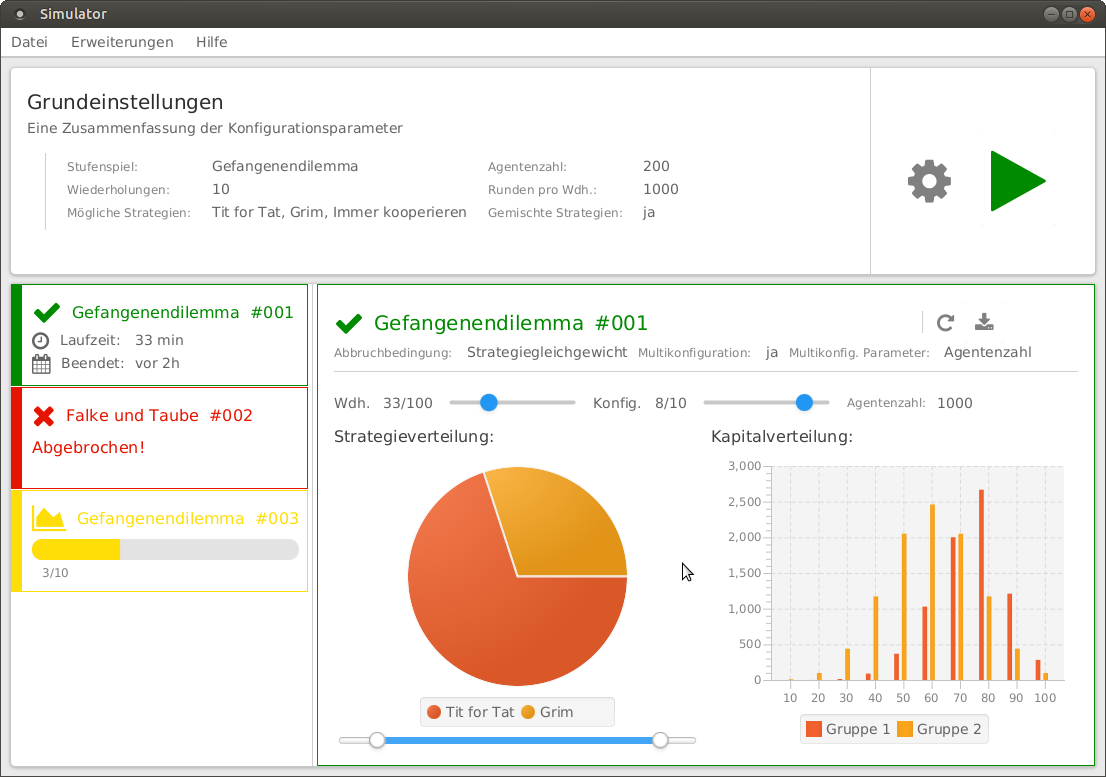
\includegraphics[width=\textwidth]{images/home.png}
	\caption{\label{fig:home}
		Hauptfenster des Simulators}
\end{figure}

Im oberen Drittel des Fensters wird eine Zusammenfassung der aktuell ausgewählten Konfiguration angezeigt (siehe \cref{fig:home_top}). Rechts davon befindet sich ein Knopf zum Bearbeiten der Konfiguration und ein weiterer Knopf zum Starten der Simulation (siehe \cref{fig:main_btn}).

\begin{figure}[hb]
	\centering
	
\includegraphics[width=\textwidth]{images/home_top.png}
	\caption{\label{fig:home_top}
	Zusammenfassung der aktuell gewählten Konfiguration}
\end{figure}

\begin{figure}[ht]
	\centering
 	
\includegraphics[width=0.25\linewidth]{images/main_btn.png}
 	\caption{\label{fig:main_btn}
 		Knöpfe zum Konfigurieren und Starten einer Simulation}
\end{figure}


\newpage
Im unteren Teil des Fenster befindet sich links eine Historie der gelaufenen, abgebrochenen und noch laufenden Simulationen (siehe \cref{fig:history}). Wird ein Eintrag angeklickt, erscheint rechts eine Zusammenfassung der Ergebnisse der ausgewählten Simulation. Mit den Knöpfen (siehe \cref{fig:out_btn}) kann die Simulation wiederholt werden oder die verwendete Konfiguration als Datei exportiert werden. Die Ausgabe besteht aus drei Seiten, zwischen denen beliebig gewechselt werden kann.Die erste Seite zeigt eine detailierte Aufführung der Strategie- und Kapitalverteilung zu jeder Wiederholung (siehe \cref{fig:home_out_1}). Die zweite Seite zeigt in einer abstrahierten Ausgabe die \Gls{Effizienz} und die \Gls{Einstellungsdauer} von Gleichgewichten (siehe \cref{fig:home_out_2}). Im Falle einer Multikonfiguration wird auf der dritten Seite eine abstrahierte Ausgabe in Abhängigkeit des multikonfigurationsparameter gezeigt (siehe \cref{fig:home_out_3}).



\begin{figure}[hb]
	\centering
	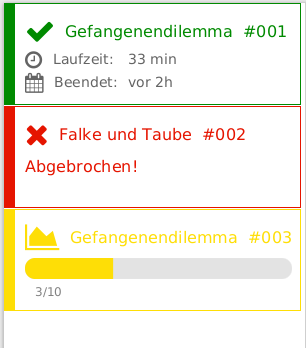
\includegraphics[height=0.5\linewidth ]{images/history.png}
	\caption{\label{fig:history}
		Simulationshistorie }
\end{figure}

\begin{figure}[ht]
	\centering
	
\includegraphics{images/out_btn.png}
	\caption{\label{fig:out_btn}
		Knöpfe zum Wiederholen und Exportieren der Ergebnisse einer Simulation}
\end{figure}
\begin{figure}[H]
	\centering
	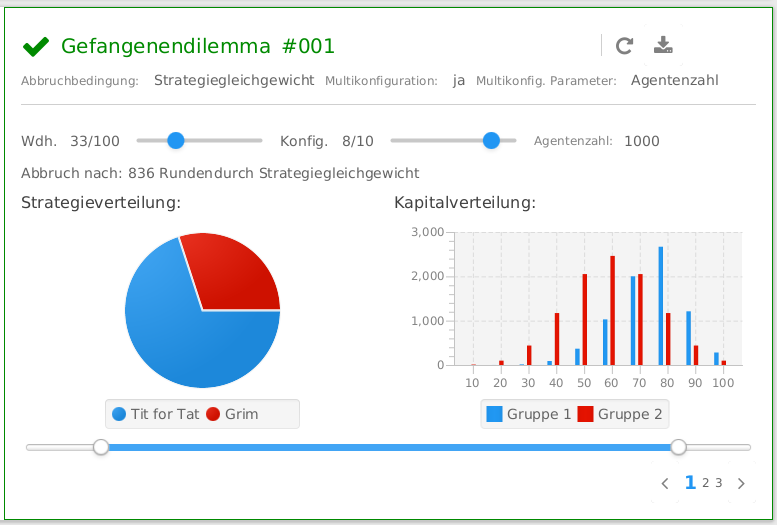
\includegraphics[width=0.9\textwidth]{images/home_out_1.png}
	\caption{\label{fig:home_out_1}
		Detailierte Ausgabe der Ergebnisse einer Simulation}
\end{figure}
\begin{figure}[H]
	\centering
	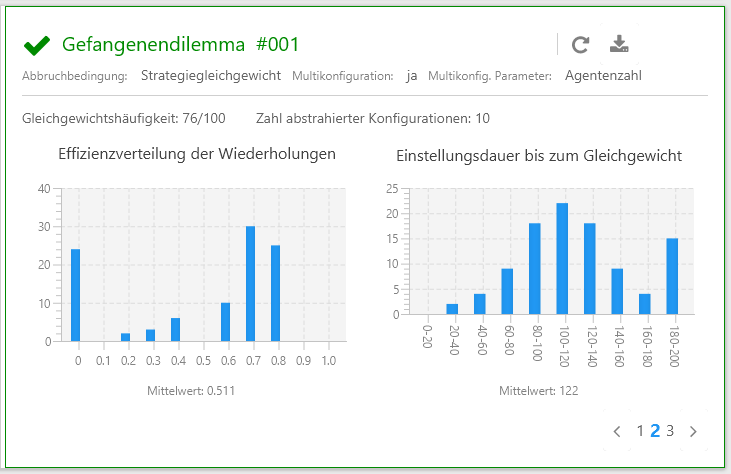
\includegraphics[width=0.9\textwidth]{images/home_out_2.png}
	\caption{\label{fig:home_out_2}
		Detailierte Ausgabe der Ergebnisse einer Simulation}
\end{figure}
\begin{figure}[H]
	\centering
	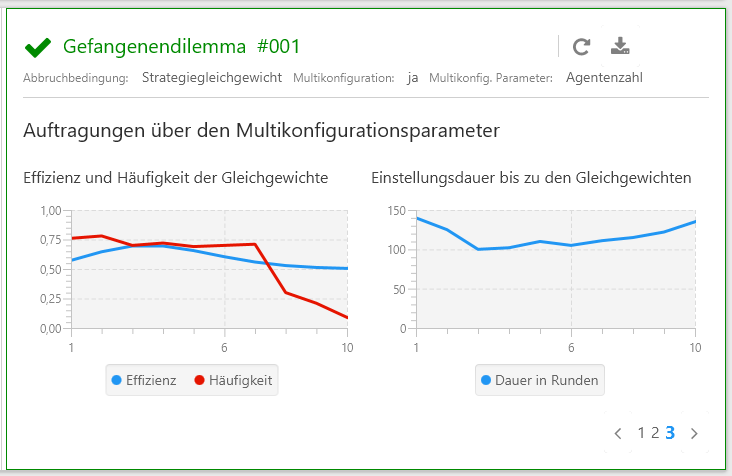
\includegraphics[width=\textwidth]{images/home_out_3.png}
	\caption{\label{fig:home_out_3}
		Detailierte Ausgabe der Ergebnisse einer Simulation}
\end{figure}

Über das Dateinmenü in der Menüleiste können Konfigurationen bearbeitet, gespeichert und geladen oder eine Simulation gestartet werden (siehe \cref{fig:menu1}).
Das Erweiterungsmenü enthält Optionen zum erstellen eines neuen Stufenspiels oder einer neuen \Gls{Strategie} (siehe \cref{fig:menu2}). Im Hilfemenü finden sich Bedienhilfen und Informationen über den Simulator (siehe \cref{fig:menu3}).

\begin{figure}[ht]
	\centering
	\subfloat[Dateimenü
	\label{fig:menu1}]{%
		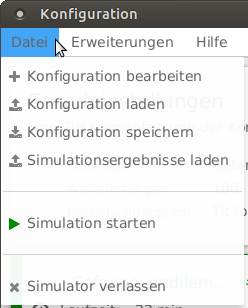
\includegraphics[height=0.25\linewidth]{images/Menu1.png}}
	\qquad
	\subfloat[Erweiterungsmenü
	\label{fig:menu2}]{%
		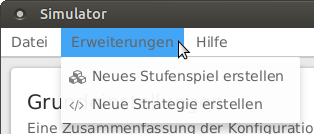
\includegraphics[width=0.25\linewidth]{images/Menu2.png}}
	\qquad
	\subfloat[Hilfemenü
	\label{fig:menu3}]{%
		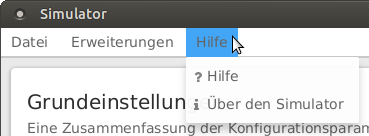
\includegraphics[width=0.25\linewidth]{images/Menu3.png}}
	\caption{\label{fig:menu}
		Funktionen der Menüleiste
	}
\end{figure}
\newpage
Drückt man den Knopf zum Bearbeiten einer Konfiguration, öffnet sich das Konfigurationsfenster (siehe \cref{fig:konfig}).

\begin{figure}[ht]
	\centering
	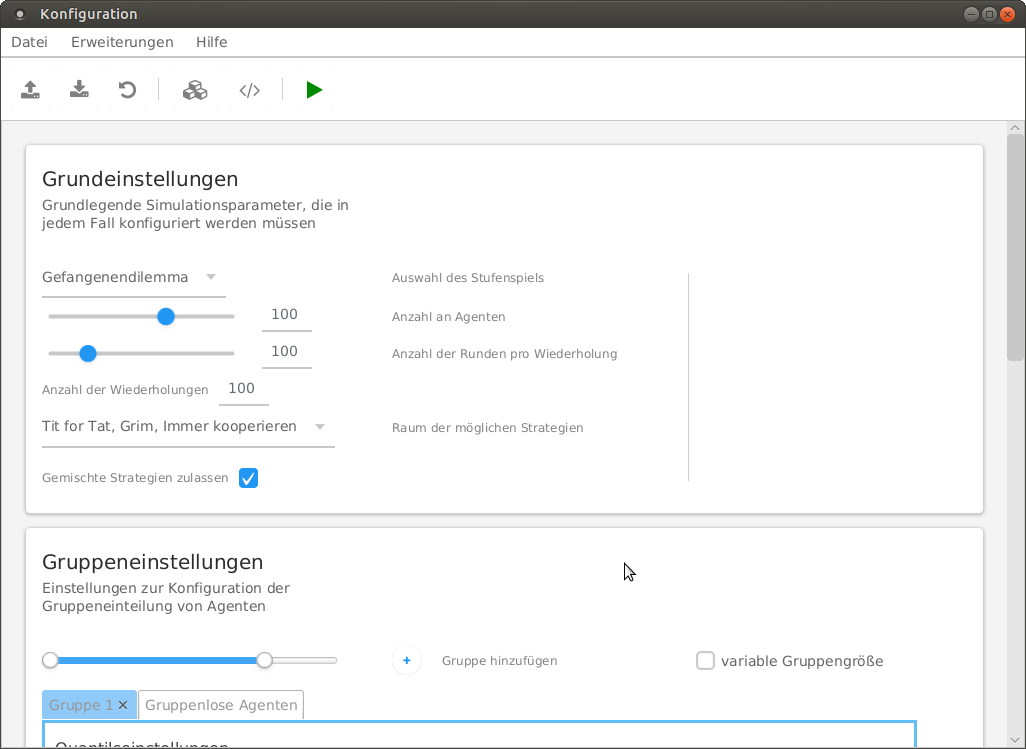
\includegraphics[width=\textwidth]{images/konfig.png}
	\caption{\label{fig:konfig}
		Konfigurationsfenster}
\end{figure}

Das Konfigurationsfenster ist in drei Bereiche unterteilt, die jeweils ein- und ausgeklappt werden können:
\begin{itemize} \itemsep -10pt
	\item Grundeinstellungen
	\item Gruppeneinstellungen
	\item Erweiterte Einstellungen
\end{itemize}

GrundEinstellungen konfigurieren die fundamentalsten Simulationsparameter. Im rechten Teil wird das ausgewählte Stufenspiel in Normalform als Bimatrix dargestellt (siehe \cref{fig:konfig_main}). Über ein spezielles Dropdownmenü mit Checkboxen können für die Simulation zugelassene \Glspl{Strategie} ausgewählt werden (siehe \cref{fig:konfig_strat_detail}).

\begin{figure}[ht]
	\centering
	
\includegraphics[width=0.25\textwidth]{images/konfig_strat_detail.png}
	\caption{\label{fig:konfig_strat_detail}
		Auswahl der zugelassenen \Glspl{Strategie}}
\end{figure}

\begin{figure}[ht]
	\centering
	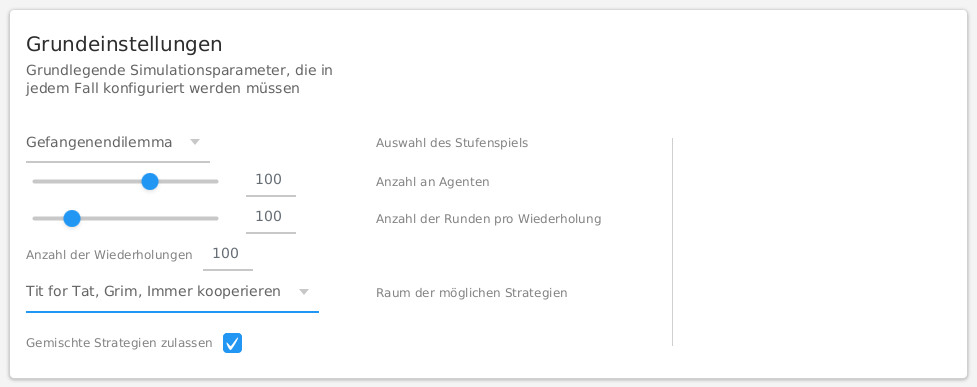
\includegraphics[width=\textwidth]{images/konfig_main.png}
	\caption{\label{fig:konfig_main}
		Grundeinstellungen im Konfigurationsfenster}
\end{figure}
\newpage
In den Gruppeneinstellungen können Gruppen angelegt und mit einem \Gls{Multislider} die Agenten frei in diese verteilt werden. Für jede Gruppe gibt es einen Tab (siehe \cref{fig:konfig_group}). Dort kann die Gruppe in gleicher Weise weiter in Segmente eingeteilt werden. Für jedes Segment kann das Startkapital der Agenten gemäß einer gewählten Verteilung festgelegt werden (siehe \cref{fig:konfig_cap} und die Initialstrategien eingestellt werden (siehe \cref{fig:konfig_strat}).



\begin{figure}[ht]
	\centering
	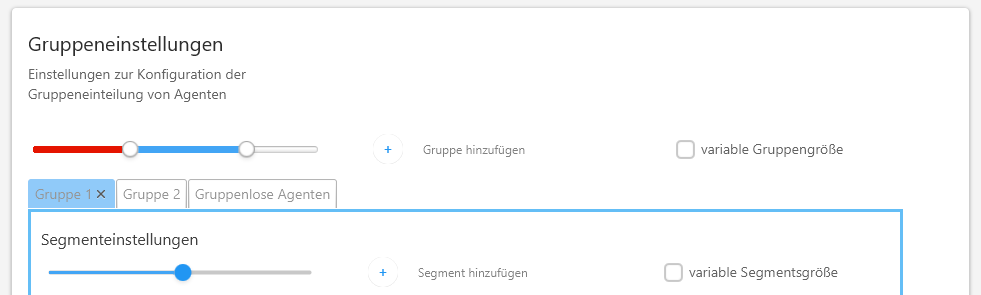
\includegraphics[width=\textwidth]{images/konfig_group.png}
	\caption{\label{fig:konfig_group}
		Gruppeneinstellungen im Konfigurationsfenster}
\end{figure}


In den erweiterten Einstellungen können spezialisierte Konfigurationen per Dropdowns eingestellt werden. Zudem kann hier der variable Konfigurationsparameter eingestellt werden, falls dieser in den Gruppen- bzw. SegementEinstellungen ausgewählt wurde. Dazu wird ein prozentualer Start- und Endwert angegeben und eine Schrittweite festgelegt \\(siehe \cref{fig:konfig_adv}). Hierdurch wird eine Multikonfiguration erstellt.

Am oberen Rand des Konfigurationsfenster befindet sich das gleiche Menü wie beim Hauptfenster (siehe \cref{fig:menu}) und darunter eine Werkzeugleiste (siehe \cref{fig:konfig_tool}). Über die Werkzeugleiste ist es möglich, Konfigurationen zu laden, zu speichern und die aktuelle Konfiguration auf die Standardwerte zurückzusetzen.\\Darüber hinaus gibt es hier Knöpfe zum Erstellen neuer Stufenspiele und \Glspl{Strategie}. Eine Simulation mit der gewählten Konfiguration kann über die Werkzeugleiste gestartet oder das Konfigurationsfenster verlassen werden.

\begin{figure}[hb]
	\centering
	
\includegraphics[width=0.5\textwidth]{images/konfig_tool2.png}
	\caption{\label{fig:konfig_tool}
		Werkzeugleiste des Konfigurationsfenster}
\end{figure}

\begin{figure}[hb]
	\centering
	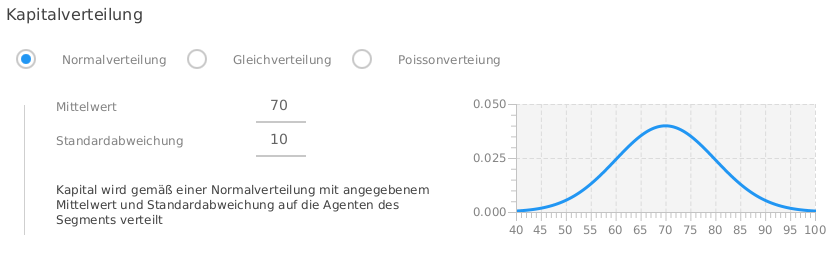
\includegraphics[width=\textwidth]{images/konfig_cap.png}
	\caption{\label{fig:konfig_cap}
		Auswahl der Kapitalverteilung für ein Segment}
\end{figure}

\begin{figure}[hb]
	\centering
	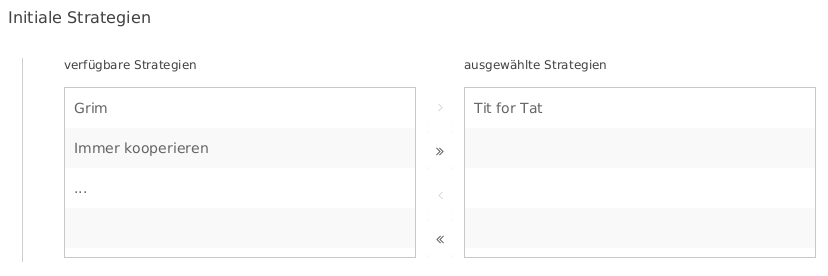
\includegraphics[width=\textwidth]{images/konfig_strat.png}
	\caption{\label{fig:konfig_strat}
		Auswahl der möglichen Initialstrategien für ein Segment}
\end{figure}

\newpage


Die Option zum Erstellen einer neuen \Gls{Strategie} öffnet ein neues Fenster (siehe \cref{fig:strategy}). Hier können vorgegebene Bedingungen mit logischen Operatoren zu einem logischen Ausdruck verknüpft werden. Einzelne Aspekte der Bedingungen können angepasst werden (siehe \cref{fig:strategy_drop}). Per Dropdown werden die Aktionen gewählt, die nach Auswertung des Ausdrucks angewendet werden.


\begin{figure}[hb]
	\centering
	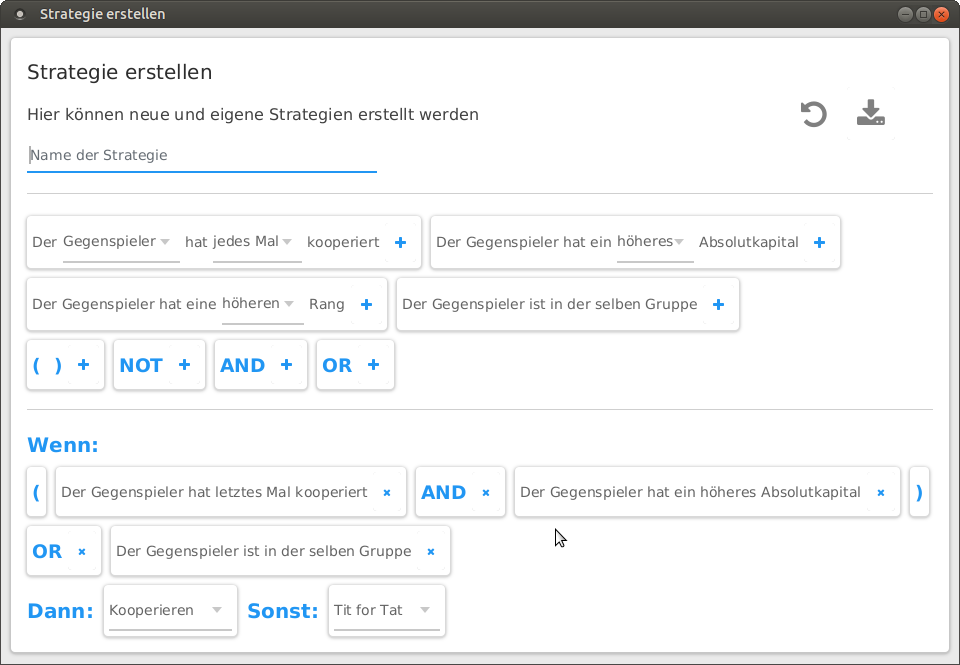
\includegraphics[width=\textwidth]{images/strategy.png}
	\caption{\label{fig:strategy}
		Erstellung einer neuen \Gls{Strategie}}
\end{figure}


\begin{figure}[hb]
	\centering
	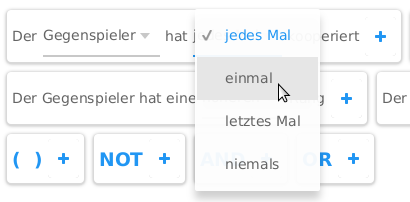
\includegraphics[width=0.5\textwidth]{images/strategy_drop.png}
	\caption{\label{fig:strategy_drop}
		Anpassung von Bedingungen}
\end{figure}

Die Wahl der Option zum Ersellen eines neuen Stufenspiels öffnet ebenfalls ein neues Fenster (siehe \cref{fig:new_game}). Ein neues Spiel wird in seiner Normalform in die gegebene Bimatrix eingetragen.

\begin{figure}[ht]
	\centering
	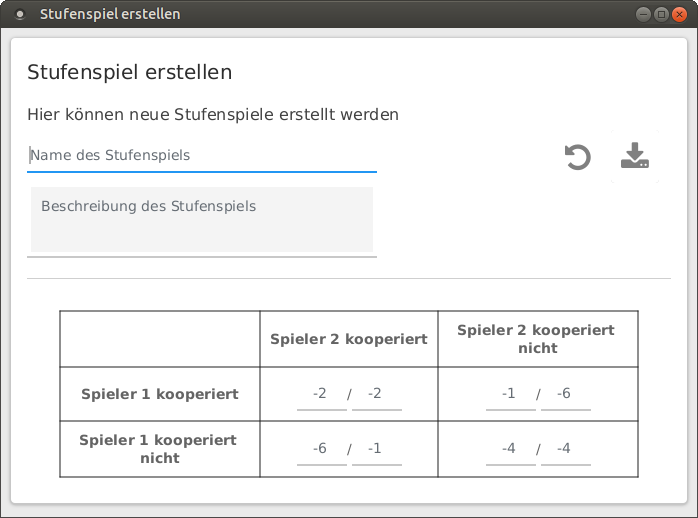
\includegraphics[width=\textwidth]{images/game.png}
	\caption{\label{fig:new_game}
		Erstellung eines neuen Stufenspiels}
\end{figure}


\begin{figure}[hb]
	\centering
	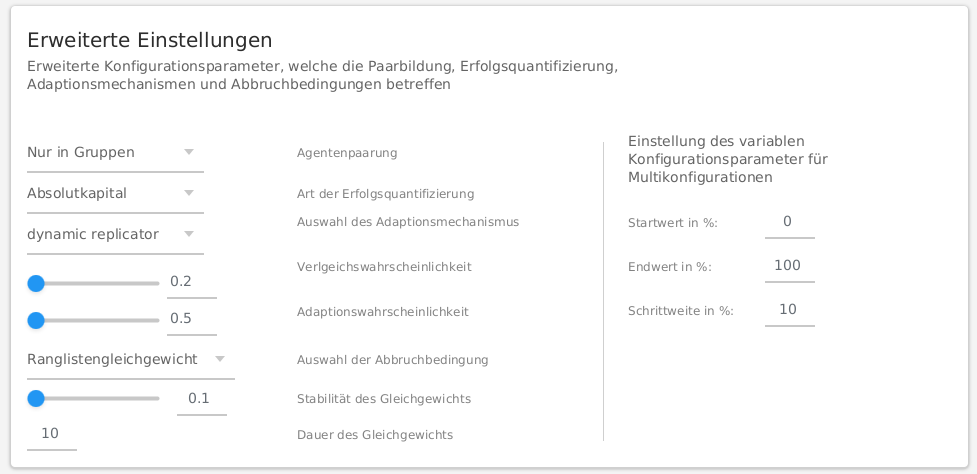
\includegraphics[width=\textwidth]{images/konfig_adv.png}
	\caption{\label{fig:konfig_adv}
		erweiterte Simulationsparameter und MultikonfigurationsEinstellungen}
\end{figure}


\section{Szenarien}


\subsection{Szenario 1}
Jonas hat die Anwendung auf seinem PC installiert und möchte das Stufenspiel Gefangenendilemma mit 10 Agenten simulieren, wobei von Anfang an eine Hälfte arm und eine Hälfte reich sein soll. Dazu öffnet Jonas die Anwendung und landet im Hauptfenster. Jonas drückt auf das Zahnrad um die von ihm gewünschte Konfiguration einzustellen. Das Konfigurationsfenster öffnet sich und Jonas wählt nun \enquote{Gefangenendilemma} bei der Auswahl des Stufenspiel aus und stellt den Slider bei Anzahl der Agenten auf 10. Die Anzahl der Runden und Wiederholungen lässt er auf den voreingestellten Werten.
Um die Agenten jetzt in 2 Gruppen einzuteilen, erstellt Jonas unter Gruppeneinstellungen 2 neue Gruppen in dem er 2 mal auf das Plus mit \enquote{Gruppe hinzufügen} klickt. Er versetzt den \Gls{Multislider} nun so, dass in der einen Gruppe 6 Agenten sind und in der anderen Gruppe 4. Er klickt auf den Bereich des \Gls{Multislider} der an Gruppe 1 zugeteilt wurde und stellt im Unterpunkt Kapitalverteilung eine Normalverteilung mit Mittelwert 200 und Standardabweichung 5 ein. Gleiches tut er für Gruppe 2, jedoch wählt er hier als Mittelpunkt 40. Für beide Gruppen wählt er unter Strategieeinteilung nur \enquote{Grim}.
Jonas ist zufrieden mit seiner Konfiguration und startet diese nun mit einem Klick auf den grünen Play-Button in der Header-Leiste.
Er wird zurück ins Hauptfenster navigiert und sieht seine Simulation nun in der Simulationshistorie. Sie ist gelb eingefärbt (Sie läuft noch. Nach einer halben Stunde schaut Jonas noch mal nach, seine Simulation ist jetzt grün eingefärbt (Sie ist beendet). Mit einem Klick auf die Simulation öffnet Jonas die Zusammenfassung für seine Simulation und schaut sich nun die Kapitalverteilung für die einzelnen Gruppen an und wertet sie aus. Jonas ist zufrieden mit seinem Ergebnis und schließt die Anwendung wieder.


\subsection{Szenario 2}

Bob möchte eine Simulation des \enquote{Falke und Taube}-Stufenspiel mit 20 Agenten durchführen und die Verteilung der 2 Anfangsstrategien \enquote{Immer Kooperation} und Nie Kooperation so variieren lassen, dass in der ersten Simulation 10\% \enquote{Immer Kooperation} und 90\% \enquote{Nie Kooperation} als Anfangsstrategie haben und diese Verteilung sich in jeder Simulation um 10\% verschiebt(20:80, 30:70...). Dazu startet Bob die Anwendung und wählt das dementsprechende Stufenspiel und die Agentenzahl in den Grundeinstellungen. Den Raum der \Glspl{Strategie} hat er auf \enquote{Nie Kooperation} und \enquote{Immer Kooperation} eingestellt und kann nun in den erweiterten Einstellungen seine Einstellung für den variablen Konfigurationsparameter treffen. Er stellt den Startwert auf 10\%, den Endwert auf 90\% und die Schrittweite auf 10\%. Er bestätigt die Konfiguration in dem er auf den grünen Haken in der Headerleiste klickt und gelangt zurück zum Hauptfenster. Im Hauptfenster kann er sich noch einmal die Zusammenfassung seiner aktuellen Konfiguration anschauen und überprüft ob er die wichtigen Dinge eingestellt hat. Nachdem er sich davon überzeugt hat, klickt er auf den grünen Play-Button um die Simulation zu starten. Er kann jetzt in der Simulationshistorie verfolgen wie viele von seinen 9 Simulationen schon beendet wurden. Nachdem alle Simulationen beendet sind, klickt er auf die Simulationsgruppe und kann sich nun eine Abstraktion der Simulationen anzeigen lassen um den Einfluss, den die Variation seines Parameter auf das Endergebnis hatte, auszuwerten. Bob findet ,dass diese eine interessante Auswirkung auf die Kapitalverteilung hatte und will die Konfiguration speichern um die Simulationen nächste Woche noch einmal durchzuführen. Dazu klickt er unter \enquote{Datei} auf \enquote{Konfiguration speichern} und kann nun einen Ablageort auswählen. Nach dem Speichern, schließt Bob die Anwendung und schickt die Konfigurationsdatei per E-Mail an seinen Kollegen Jonas, damit dieser die Simulation auch starten kann. Jonas kann die Konfiguration mittels \enquote{Konfiguration laden} öffnen und dann ganz normal starten.

\newpage

\section{Stufenspiele}
Im folgenden findet sich eine kurze Beschreibung der verfügbaren Stufenspiele.

\textbf{Gefangenendilemma:}
Zwei Verdächtige werden ohne vorherige Absprachen getrennt voneinander verhört. Beide haben die Möglichkeit das Verbrechen zu gestehen und damit den anderen zu verraten, oder zu schweigen. Die Dauer ihrer Haftstrafe hängt von ihrer eigenen Aussage und der Aussage des anderen ab.
\begin{table}[ht]
\center
	\begin{tabular}{|c|c|c|c|c|c|}
		\cline{1-6}
		\multicolumn{2}{|c|}{} & \multicolumn{4}{ c| }{Spieler 2} \\ \cline{3-6}
		\multicolumn{2}{|c|}{} & \multicolumn{2}{c|}{schweigt} & \multicolumn{2}{c|}{gesteht} \\ \cline{1-6}
		\multirow{2}{*}{Spieler 1} & schweigt & -2 & -2 & -6 & -1  \\ \cline{2-6}
		& \multicolumn{1}{ |c| }{gesteht} & -1 & -6 & -4 & -4 \\ \cline{1-6}

	\end{tabular}

\caption{Normalform Gefangenendilemma}

\end{table}

\textbf{Hirschjagd:}
Zwei Jäger befinden sich auf der Hirschjagd. Es kommt ein Hase vorbei und beide haben die Wahl: Entweder sie schießen den Hasen bevor es der andere tut und vergeben die Chance auf das gemeinsame erlegen eines Hirschs, oder sie geben die Gelegenheit nicht her und laufen Gefahr weder Hasen noch Hirsch zu bekommen.
\begin{table}[ht]
	\center
	\begin{tabular}{|c|c|c|c|c|c|}
	\cline{1-6}
	\multicolumn{2}{|c|}{} & \multicolumn{4}{ c| }{Spieler 2} \\ \cline{3-6}
	\multicolumn{2}{|c|}{} & \multicolumn{2}{c|}{Hirschjagd} & \multicolumn{2}{c|}{Hasenjagd} \\ \cline{1-6}
	\multirow{2}{*}{Spieler 1} & Hirschjagd & 4 & 4 & 0 & 3  \\ \cline{2-6}
	& \multicolumn{1}{ |c| }{Hasenjagd} & 3 & 0 & 3 & 3 \\ \cline{1-6}
\end{tabular}

	\caption{Normalform Hirschjagd}

\end{table}

\textbf{Feiglingsspiel:}
Wegen einer Mutprobe rasen zwei Personen mit Autos aufeinander zu. Wer Ausweicht, gilt gegenüber dem andere als Feigling und hat die Wette verloren. Weicht keiner von beiden aus, verlieren sie bei der Kollision ihr Leben.
\begin{table}[ht]
	\center
	\begin{tabular}{|c|c|c|c|c|c|}
	\cline{1-6}
	\multicolumn{2}{|c|}{} & \multicolumn{4}{ c| }{Spieler 2} \\ \cline{3-6}
	\multicolumn{2}{|c|}{} & \multicolumn{2}{c|}{Ausweichen} & \multicolumn{2}{c|}{Weiterfahren} \\ \cline{1-6}
	\multirow{2}{*}{Spieler 1} & Ausweichen & 4 & 4 & 2 & 6  \\ \cline{2-6}
	& \multicolumn{1}{ |c| }{Weiterfahren} & 6 & 2 & 0 & 0 \\ \cline{1-6}
\end{tabular}

	\caption{Normalform Feiglingsspiel}

\end{table}
\newpage
\textbf{Kampf der Geschlechter:}
Ein Mann und eine Frau wollen zusammen ausgehen, haben aber keinen Treffpunkt vereinbart. Zur Wahl steht entweder ein Fußballspiel oder ein Konzert. Beide müssen sich entscheiden mit der Gefahr sich nicht zu treffen. Der Mann bevorzugt das Fußballspiel, während die Frau lieber auf das Konzert geht.
\begin{table}[ht]
	\center
	\begin{tabular}{|c|c|c|c|c|c|}
	\cline{1-6}
	\multicolumn{2}{|c|}{} & \multicolumn{4}{ c| }{Spieler 2} \\ \cline{3-6}
	\multicolumn{2}{|c|}{} & \multicolumn{2}{c|}{Fußball} & \multicolumn{2}{c|}{Konzert} \\ \cline{1-6}
	\multirow{2}{*}{Spieler 1} & Fußball & 3 & 1 & 0 & 0  \\ \cline{2-6}
	& \multicolumn{1}{ |c| }{Konzert} & 0 & 0 & 1 & 3 \\ \cline{1-6}
\end{tabular}

	\caption{Normalform Kapf der Geschlechter}

\end{table}

\textbf{Vertrauensspiel:}
Ein Treugeber kann einem Treuhänder eine Aufgabe betrauen. Entscheidet sich der Treugeber dem Treuhänder nicht zu vertrauen, so kommt kein Geschäft zustande. Anderenfalls hat dr Treuhänder die Möglichkeit das ihm entgegengebrachte Vertrauen zu missbrauchen, oder zu honorieren.
\begin{table}[ht]
	\center
	\begin{tabular}{|c|c|c|c|c|c|}
	\cline{1-6}
	\multicolumn{2}{|c|}{} & \multicolumn{4}{ c| }{Spieler 2} \\ \cline{3-6}
	\multicolumn{2}{|c|}{} & \multicolumn{2}{c|}{Missbrauch} & \multicolumn{2}{c|}{Honorierung} \\ \cline{1-6}
	\multirow{2}{*}{Spieler 1} & vertrauen & -1 & 2 & 1 & 1  \\ \cline{2-6}
	& \multicolumn{1}{ |c| }{nicht vertrauen} & 0 & 0 & 0 & 0 \\ \cline{1-6}
\end{tabular}

	\caption{Normalform Vertrauensspiel}

\end{table}

\textbf{Elfmeterschießen:}
Beim Elfmeterschießen müssen sich Schütze und Torwart zwischen der linken und der rechten Torhälfte entscheiden. Dabei will der Torwart die gleiche Seite wählen wie der Schütze, um den Ball zu halten und der Schütze möchte eine andere Seite wählen als der Torwart, um ein Tor zu erziehlen.
\begin{table}[ht]
	\center
	\begin{tabular}{|c|c|c|c|c|c|}
	\cline{1-6}
	\multicolumn{2}{|c|}{} & \multicolumn{4}{ c| }{Spieler 2} \\ \cline{3-6}
	\multicolumn{2}{|c|}{} & \multicolumn{2}{c|}{links} & \multicolumn{2}{c|}{rechts} \\ \cline{1-6}
	\multirow{2}{*}{Spieler 1} & links & 3 & 1 & 0 & 0  \\ \cline{2-6}
	& \multicolumn{1}{ |c| }{rechts} & 0 & 0 & 1 & 3 \\ \cline{1-6}
\end{tabular}

	\caption{Normalform Elfmeterschießen}

\end{table}
\newpage

\printnoidxglossaries

\end{document}
